% Computational Mechanics: Springer Nature editable review manuscript.
% Single-column review layout; the journal recommends iicol for final layout.
\documentclass[pdflatex,sn-basic,Numbered]{sn-jnl}

\usepackage{amsmath,amssymb}
\usepackage{booktabs}
\usepackage{float}
\usepackage{subcaption}
\captionsetup[figure]{name=Fig.,labelfont=bf,labelsep=space}
\usepackage{tabularx}
\usepackage{siunitx}
\usepackage{graphicx}
\usepackage{tikz}
\usetikzlibrary{arrows.meta,positioning,shapes.geometric,fit,backgrounds,%
  decorations.pathreplacing,calligraphy}

\newcounter{algorithm}
\renewcommand{\thealgorithm}{\arabic{algorithm}}

\newenvironment{algorithm}[1][]{%
  \refstepcounter{algorithm}%
  \par\medskip
  \noindent
  \hrule
  \vspace{0.45em}
  \def\caption##1{%
    \textbf{Algorithm~\thealgorithm.} ##1\par
    \vspace{0.45em}%
  }%
}{%
  \par
  \vspace{0.2em}
  \hrule
  \par\medskip
}

\graphicspath{{figures/}}
\setlength{\emergencystretch}{3em}

\hypersetup{
  colorlinks=true,
  linkcolor=blue,
  citecolor=blue,
  urlcolor=blue,
  pdftitle={Efficient affine operator compilation for reduced-order elastic homogenization of voxelized composites},
  pdfauthor={Kevin Vidal, Victor Alulema, Victor Berrazueta, Esteban Valencia},
  pdfsubject={Affine operator compilation for reduced-order elastic homogenization},
  pdfkeywords={computational homogenization, reduced basis, affine operators, elastic composites}
}

\newcommand{\R}{\mathbb{R}}
\newcommand{\G}{\mathcal{G}}

\newcommand{\Heff}{H^{\mathrm{eff}}}
\newcommand{\Hr}{H^{\mathrm{eff}}_r}
\newcommand{\Hfom}{H^{\mathrm{eff}}_{\mathrm{FOM}}}

\newcommand{\Ceff}{C^{\mathrm{eff}}}
\newcommand{\Cr}{C^{\mathrm{eff}}_r}
\newcommand{\Cfom}{C^{\mathrm{eff}}_{\mathrm{FOM}}}

\begin{document}

\renewcommand{\bibfont}{\normalsize}
\title[Affine compilation for elastic homogenization]{Efficient affine operator
compilation for reduced-order elastic homogenization of voxelized composites}

\author*[1]{\fnm{Kevin} \sur{Vidal}}\email{kevin.vidal@epn.edu.ec}
\author[1,2]{\fnm{Victor} \sur{Alulema}}
\author[1]{\fnm{Victor} \sur{Berrazueta}}
\author[1]{\fnm{Esteban} \sur{Valencia}}

\affil[1]{\orgdiv{Department of Mechanical Engineering; LUAS-EPN; ATA-EPN Research Group},
  \orgname{Escuela Polit\'ecnica Nacional},
  \orgaddress{\city{Quito}, \postcode{170143}, \country{Ecuador}}}
\affil[2]{\orgdiv{EAVISE, PSI, Department of Electrical Engineering (ESAT)},
  \orgname{KU Leuven}, \orgaddress{\street{Jan Pieter de Nayerlaan 5},
  \city{Sint-Katelijne-Waver}, \country{Belgium}}}

\abstract{
Repeated computational homogenization becomes prohibitively expensive when a
resolved microstructure must be evaluated over many combinations of
constituent properties. This work develops an efficient affine operator
compiler for reduced-order linear elastic homogenization on voxel grids.
Microscopic strain snapshots from a fast Fourier transform solver generate
Galerkin spaces; phase-supported constitutive factors, incremental cross-block
contractions, and reuse of the projected reference metric reduce the cost of
forming their operators. The compiler supports both complete snapshot spaces
and proper orthogonal decomposition, which share the same reduced Schur
output map. Established variational identities provide energy diagnostics
relative to the discrete full-order model. Across ten short-fiber composite
microstructures with up to \(240^3\) voxels, 6--16 training materials plus
five monitoring materials give reduced ranks of 36--96. Validation on
20 unseen materials shared across the ten geometries yields mean and maximum
relative stiffness errors of \(0.0217\%\) and \(0.1322\%\).
A separate controlled comparison shows complete construction times of
30.66 and 159.41 seconds for two larger cells, reductions of 21.2 and
31.4 percent relative to the tested conventional compilation path; no
reduction is observed for the smallest cell. Energy-based proper orthogonal
decomposition obtains smaller ranks at nearly the same construction cost.
Measured isolated reduced queries on a central processing unit take
21.18--47.83 microseconds. These results support efficient operator assembly
as the computational contribution, with benefits that depend on cell size,
retained rank, and the numerical accuracy of the contracted operators.
}

\keywords{Computational homogenization, Affine operator compilation,
Reduced basis, Proper orthogonal decomposition, FFT methods, Elastic composites}

\maketitle

\section*{Nomenclature}

\begingroup
\scriptsize
\renewcommand{\arraystretch}{1.08}
\setlength{\tabcolsep}{4pt}
\noindent\begin{tabularx}{\textwidth}{@{}lXlX@{}}
\toprule
Symbol & Meaning & Symbol & Meaning \\
\midrule

\multicolumn{4}{@{}l}{\textit{General formulation}} \\
\addlinespace[1mm]

\(\Omega,\boldsymbol{x},|\Omega|\) &
Periodic cell, spatial coordinate, and cell volume. &
\(\G\) &
Fixed discrete microstructure, including phase layout, orientations, and grid. \\

\(\boldsymbol{\xi},\Xi,\boldsymbol{\xi}^{\star}\) &
Constitutive-parameter vector, admissible domain, and queried point. &
\(g,g_i,m\) &
Macroscopic loading vector, loading amplitudes, and number of independent loadings. \\

\(\overline{\boldsymbol z}_i,\overline{\boldsymbol z}(g)\) &
Unit macroscopic driving states and their combination. &
\(\boldsymbol z(\boldsymbol x;g)\) &
Local microscopic field. \\

\(\mathcal V_{\mathrm{per}},\mathcal V_{\mathrm{per}}^h\) &
Continuous and discrete admissible periodic zero-mean fluctuation spaces. &
\(u,u_g,v\) &
Microscopic fluctuation, equilibrium fluctuation, and test function. \\

\(\mathcal L\) &
Microscopic differential operator. &
\(\phi_a,\phi_b\) &
Basis functions of \(\mathcal V_{\mathrm{per}}^h\). \\

\(\mathbb A,\mathbb A_q\) &
Local constitutive operator and fixed-microstructure affine fields. &
\(\Heff,\Hfom,\Hr\) &
Continuum, full-order, and reduced effective operators; \(r\) denotes the Ritz rank. \\

\(\mathcal E\) &
Volume-normalized quadratic energy. &
\(n\) &
Number of independent microscopic unknowns in the constrained discrete space
\(\mathcal V_{\mathrm{per}}^h\). \\

\(K,B,D\) &
Microscopic, coupling, and macroscopic energy blocks. &
\(X=[X_1,\ldots,X_m]\) &
Full-order response matrix satisfying \(KX=B\). \\

\(Q,\gamma_q,\boldsymbol\gamma\) &
Number of affine terms, affine constitutive coefficient, and coefficient vector. &
\(\|\cdot\|_F\) &
Frobenius norm. \\

\(\succeq,\preceq\) &
Loewner ordering for symmetric matrices. &
\(\mathrm{FOM},\mathrm{ROM}\) &
Full-order and reduced-order models. \\

\(k,\sigma_e,\mathsf d,\varepsilon,\kappa\) &
Thermal conductivity, electrical conductivity, diffusivity, permittivity, and permeability. &
\(\boldsymbol{\sigma},\boldsymbol{\varepsilon}(\cdot)\) &
Elastic stress and symmetric-gradient operator. \\

\(N_{\mathrm{vox}}\) &
Total voxel count; the three-dimensional strain-based implementation stores
six microscopic field components per voxel. & & \\

\bottomrule
\end{tabularx}

\par\medskip
\noindent\begin{tabularx}{\textwidth}{@{}lXlX@{}}
\toprule
Symbol & Meaning & Symbol & Meaning \\
\midrule

\multicolumn{4}{@{}l}{\textit{Sobol--Ritz construction and validation}} \\
\addlinespace[1mm]

\(\Xi_C,N_C\) &
Sobol candidate sequence and its size. &
\(\Xi_S,N_s\) &
Selected training prefix of \(\Xi_C\) and its size. \\

\(\Xi_M,N_M\) &
Independent monitor set and its size. &
\(\Xi_V,N_V\) &
Independent held-out validation set and its size. \\

\(S,S_\ell\) &
Final and intermediate snapshot matrices. &
\(p,p_\ell\) &
Raw snapshot dimensions, \(p=mN_s\) and \(p_\ell=m\ell\). \\

\(r,V_r\) &
Final Ritz rank and reference-energy Ritz basis. &
\(\widetilde K_q,\widetilde B_q\) &
Affine blocks in raw snapshot coordinates. \\

\(K_{\mathrm{ref}},G_{\mathrm{ref}},R_{\mathrm{ref}}\) &
Reference operator, reference-energy Gram matrix, and Cholesky factor. &
\(K_{q,r},B_{q,r}\) &
Precompiled reduced affine blocks. \\

\(K_r,B_r\) &
Material-dependent reduced operators. &
\(X_r,\widehat X_r\) &
Reduced microscopic response and its reference-energy coordinates. \\

\(\widehat X_\ell^{(j)}\) &
Intermediate response coordinates in the raw snapshot basis for monitor point \(j\). &
\(\Delta X,R\) &
Microscopic response-error matrix and full-order residual. \\

\(e_M^{(\ell)},e_{V,j}\) &
Monitor error and held-out validation error. &
\(\tau_{\mathrm{ROM}},\ell,\ell_{\min}\) &
ROM tolerance, enrichment index, and first monitored prefix size. \\

\(I_{\mathrm{CG}}\) &
Representative full-order CG iteration count. & & \\

\midrule
\multicolumn{4}{@{}l}{\textit{Elasticity specialization and performance}} \\
\addlinespace[1mm]

\(\mathbb C,\Ceff,\Cfom,\Cr\) &
Local and effective stiffness tensors in Mandel notation. &
\(E_m,\nu_m\) &
Matrix Young's modulus and Poisson's ratio. \\

\(E_L,E_T\) &
Fiber longitudinal and transverse Young's moduli. &
\(G_{LT},\nu_{LT},\nu_{TT}\) &
Queried fiber shear modulus and Poisson ratios. \\

\(V_f,a_{11},a_{22},a_{33}\) &
Fiber volume fraction and orientation-tensor diagonal entries. &
\(\mathcal T(\boldsymbol x;\G)\) &
Energy-preserving Mandel rotation associated with the local fiber direction. \\

\(\lambda_{\min}(\cdot)\) &
Smallest eigenvalue of a symmetric operator. &
\(t_{\mathrm{FOM}},t_{\mathrm{ROM}}\) &
Measured time per FOM and online ROM material query. \\

\(T_{\mathrm{compile}},N_{\mathrm{BE}}\) &
Total one-time offline compilation time and break-even query count. & & \\

\bottomrule
\end{tabularx}
\endgroup

\section{Introduction}
\label{sec:introduction}

Material screening, constituent identification, and multiscale simulation
require repeated homogenization of a fixed microstructure as its constituent
properties vary. For voxelized short-fiber composites, resolving the fiber
geometry and local anisotropy can require millions of voxels. The largest
cells considered here contain \(240^3\) voxels, so a single microscopic strain
field has about 83 million stored scalar components. Reusing this spatial
information across material queries is attractive, but generating and
contracting a collection of such fields creates a substantial offline
computational and memory cost. This work addresses that cost for periodic,
linear elastic composites with fixed phase and orientation fields.

FFT-based homogenization provides an efficient full-order reference on regular
grids. Developments following the original scheme of Moulinec and Suquet
\cite{moulinec1998numerical} include accelerated iterations
\cite{eyre1999fast,michel2001augmented}, variational and Galerkin methods
\cite{brisard2012galerkin,vondrejc2014fft}, and upper--lower bounds on
homogenized properties \cite{vondrejc2015bounds}. These developments reduce
and control the cost of individual cell solutions. Many-query applications,
however, can benefit from a further offline--online decomposition that reuses
cell solutions over a constitutive parameter domain.

Reduced-basis and proper orthogonal decomposition (POD) approaches already
provide this decomposition for computational homogenization
\cite{boyaval2008homogenization,yvonnet2007r3m,fritzen2013hybrid,
hernandez2014highperformance,abdulle2014reducedhomogenization}.
Affine parameter dependence permits reduced operators and output functionals
to be assembled offline \cite{prudhomme2002reliable,quarteroni2011certified},
and reduced Schur complements eliminate internal coordinates
\cite{huynh2013scrbe}. Thus, online evaluation of an effective tensor without
voxel-field reconstruction is available to a properly implemented affine
POD/reduced-basis model. The present Schur output map is an instance of that
established Galerkin construction; it is not an alternative projection
principle. Likewise, its energy-error identity and ordering under nested
enrichment follow from standard variational arguments.

Among closely related contributions, Pham and Lee \cite{pham2025rbhm}
consider reduced-basis homogenization with variable constituent properties
for thermal and elastic periodic composites. This overlap requires the
present contribution to be identified at the level of computational
construction and verified performance, rather than through the use of
variable materials or a reduced online solve alone. Other approaches reuse
microstructural information through deep material networks
\cite{liu2019dmn,gajek2020dmn}, including component-scale applications
\cite{gajek2021fedmn,gajek2022thermomechanical}, or reduce spatial cost through
sparse sampling and low-rank field representations
\cite{kochmann2019sparsefft,vondrejc2020lowrank}. These strategies address
related costs but do not constitute numerical baselines in the present study.

The computational development examined here is a compiler from microscopic
strain snapshots to reusable affine Galerkin operators. For isotropic matrix
and transversely isotropic fiber phases, seven constitutive coefficients
separate material properties from fixed spatial factors. The compiler
contracts these factors on their phase and orientation support, streams
snapshot features within a prescribed device workspace, updates only new
and cross blocks during enrichment, and recovers the reference-energy Gram
matrix from already assembled blocks. This avoids forming global stiffness
matrices and repeating unnecessary volumetric products. The resulting
operators can retain the complete snapshot span or be transformed into POD
coordinates. Their use by both models is central to a fair assessment of the
compiler, and also limits any claim of intrinsic superiority over POD.

The numerical evidence has two parts. A campaign on ten three-dimensional
short-fiber geometries tests tensor accuracy and energetic diagnostics over a
common constitutive domain. A separate comparison on three geometries uses
matched material sequences, monitoring decisions, full-order settings, and
held-out data to separate operator compilation from basis compression. Both
compilation paths are incremental; energy POD shares the factorized compiler,
while a conventional spatial contraction path supplies an implementation
baseline for \(L^2\) POD. We report complete measured construction intervals,
isolated query latency, batched throughput, and peak memory as distinct
quantities. The results support a reduction in operator-assembly cost for the
larger cells, but do not establish the best possible implementation of every
competing method.

The scope is restricted to fixed-geometry, coercive linear elastic cell
problems. Accuracy is assessed on reserved material samples, with separate
checks of the voxel discretization and reduced operators.
Section~\ref{sec:homogenization} defines the variational and affine model;
Section~\ref{sec:transfer} details compilation, normalization, and verification;
Section~\ref{sec:numerical_assessment} presents the elastic benchmarks and
controlled reduced-basis comparison. Supporting derivations and resolution
checks are given in the appendices.

\section{General parametric periodic homogenization}
\label{sec:homogenization}

\subsection{Periodic cell problem and effective operator}
\label{subsec:cell_problem}
Let \(\Omega\) denote the periodic representative cell, namely the finite
region of the heterogeneous material that is periodically repeated to describe
the microstructure. A point within the cell is identified by
\(\boldsymbol{x}\in\Omega\), while \(|\Omega|\) denotes its volume. The symbol
\(\G\) represents the fixed microstructure, including the phase distribution,
local material orientations, and spatial discretization. Throughout one
offline--online construction, \(\G\) remains unchanged, whereas the
constitutive properties of the constituent phases are allowed to vary.

These variable material properties are collected in the parameter vector
\(\boldsymbol{\xi}=[\xi_1,\ldots,\xi_{n_\xi}]^T\in\Xi\), where each
\(\xi_i\) represents one constitutive parameter, such as a Young's modulus,
Poisson ratio, conductivity, or another material coefficient, and \(\Xi\)
denotes the admissible parameter domain. Hence, each
\(\boldsymbol{\xi}\in\Xi\) identifies one material combination to be queried
for the same fixed microstructure \(\G\).

The macroscopic loading is represented by
\(g=[g_1,\ldots,g_m]^T\in\R^m\), where \(m\) is the number of independent
macroscopic components required to characterize the effective response. Let
\(\overline{\boldsymbol z}_i\) denote the \(i\)-th unit macroscopic loading
state and \(g_i\) its amplitude. The resulting macroscopic field is defined in
Eq.~\eqref{eq:macro_field} as a linear combination of these unit states:
\begin{equation}
\label{eq:macro_field}
\overline{\boldsymbol z}(g)
=
\sum_{i=1}^{m}
g_i\overline{\boldsymbol z}_i.
\end{equation}
For three-dimensional linear elasticity,
\(\overline{\boldsymbol z}\) is the symmetric macroscopic strain, which has
six independent components, and therefore \(m=6\).

If the material inside \(\Omega\) were homogeneous,
\(\overline{\boldsymbol z}(g)\) would be sufficient to describe the local
field. In a heterogeneous medium, however, the constituent phases generally
respond differently to the same imposed macroscopic loading, causing the
field to redistribute within the cell. In linear elasticity, for example, an
imposed macroscopic strain is redistributed between the constituent phases
according to their local stiffness and orientation. This microscopic
redistribution is represented by a fluctuation field
\(u(\boldsymbol{x})\in\mathcal V_{\mathrm{per}}\), where
\(\mathcal V_{\mathrm{per}}\) denotes the space of admissible periodic
fluctuations, with the zero-mean condition in
Eq.~\eqref{eq:zero_mean} imposed to preserve the prescribed macroscopic
average:
\begin{equation}
\label{eq:zero_mean}
\frac{1}{|\Omega|}
\int_{\Omega}
u(\boldsymbol x)\,
\mathrm{d}\boldsymbol x
=
0.
\end{equation}
Periodicity enforces compatibility of the fluctuation on opposite faces of the
cell, while Eq.~\eqref{eq:zero_mean} removes its arbitrary constant component
and prevents the microscopic correction from modifying the imposed
macroscopic average.

The local field is then obtained by adding the microscopic correction to the
prescribed macroscopic field, as written in Eq.~\eqref{eq:local_field}:
\begin{equation}
\label{eq:local_field}
\boldsymbol z(\boldsymbol x;g)
=
\overline{\boldsymbol z}(g)
+
\mathcal L u(\boldsymbol x).
\end{equation}
Here, \(\mathcal L\) is the differential operator that converts the
fluctuation variable into the physical field entering the constitutive law.
For scalar transport, \(\mathcal L=\nabla\), whereas in linear elasticity
\(\mathcal L=\boldsymbol{\varepsilon}(\cdot)\). Accordingly,
Eq.~\eqref{eq:local_field} becomes
\(\boldsymbol{\varepsilon}(\boldsymbol x)
=
\overline{\boldsymbol{\varepsilon}}
+
\boldsymbol{\varepsilon}(u)\)
in elasticity, showing that the local strain consists of the prescribed
macroscopic strain plus the microscopic redistribution induced by the
heterogeneous microstructure.

Once the local field in Eq.~\eqref{eq:local_field} has been established, the
next step is to determine the physical response it produces inside the
heterogeneous cell. This response is governed by the local constitutive
operator \(\mathbb A(\boldsymbol x;\boldsymbol\xi,\G)\), which is assumed
symmetric and coercive. Symmetry means that the constitutive coupling between
two admissible local fields is unchanged when their roles are interchanged,
\(\boldsymbol z_1^T\mathbb A\boldsymbol z_2
=
\boldsymbol z_2^T\mathbb A\boldsymbol z_1\), allowing the response to be
described through a quadratic variational functional, whereas coercivity
requires every nonzero admissible local field to have a strictly positive
energetic cost, meaning that a nonzero deformation or driving field cannot
occur without storing or dissipating a positive amount of energy. Together,
symmetry and coercivity guarantee a stable and unique minimum of the
variational problem and, after discretization, lead to a symmetric
positive-definite microscopic operator; in linear elasticity, this general
constitutive operator becomes the local stiffness tensor,
\(\mathbb A=\mathbb C\), which relates the local strain obtained from
Eq.~\eqref{eq:local_field} to the corresponding stress through
\(\boldsymbol\sigma(\boldsymbol x)
=
\mathbb C(\boldsymbol x;\boldsymbol\xi,\G)
\boldsymbol\varepsilon(\boldsymbol x)\).

At this stage, Eq.~\eqref{eq:local_field}, together with the local constitutive
law, describes the response associated with any admissible fluctuation \(u\),
but it does not yet identify which fluctuation corresponds to the physical
equilibrium of the heterogeneous cell. The microscopic cell problem therefore
consists of selecting the particular fluctuation that satisfies equilibrium
for the prescribed macroscopic loading \(g\). Because the constitutive
response is linear and symmetric, this equilibrium can be characterized
variationally through a quadratic microscopic functional obtained from the
local constitutive law and the field decomposition in
Eq.~\eqref{eq:local_field}; its derivation is provided in
Appendix~\ref{app:microscopic_functional_derivation}, while the resulting
volume-averaged functional is defined in
Eq.~\eqref{eq:microscopic_energy} as
\begin{equation}
\label{eq:microscopic_energy}
\Pi(u;g,\boldsymbol{\xi},\G)
=
\frac{1}{2|\Omega|}
\int_{\Omega}
\left[
\overline{\boldsymbol z}(g)
+
\mathcal L u
\right]^T
\mathbb A(\boldsymbol x;\boldsymbol\xi,\G)
\left[
\overline{\boldsymbol z}(g)
+
\mathcal L u
\right]
\,\mathrm{d}\boldsymbol x.
\end{equation}
Equation~\eqref{eq:microscopic_energy} therefore assigns a quadratic
volume-averaged response to each candidate fluctuation \(u\); in linear
elasticity, where \(\mathbb A=\mathbb C\), this quantity is the
volume-averaged stored elastic energy of the periodic cell.

Because the symmetry and coercivity of \(\mathbb A\) make the microscopic
variational problem well posed, the physical equilibrium fluctuation is
obtained by selecting, among all admissible fields, the one that minimizes
Eq.~\eqref{eq:microscopic_energy}, with this equilibrium field denoted by
\(u_g\) and defined in Eq.~\eqref{eq:equilibrium_minimizer} as
\begin{equation}
\label{eq:equilibrium_minimizer}
u_g
=
\operatorname*{arg\,min}_{u\in\mathcal V_{\mathrm{per}}}
\Pi(u;g,\boldsymbol\xi,\G).
\end{equation}

To verify that the equilibrium field \(u_g\), defined in
Eq.~\eqref{eq:equilibrium_minimizer}, corresponds to a minimum of the
microscopic functional, consider a small admissible perturbation of this
field, \(u_g+\epsilon v\), where \(\epsilon\) controls the perturbation
magnitude and \(v\in\mathcal V_{\mathrm{per}}\) is an admissible test
function representing any virtual direction that preserves the periodicity
and zero-mean conditions of Eq.~\eqref{eq:zero_mean}. If \(u_g\) is at a
minimum, an infinitesimal perturbation in any such direction cannot change the
microscopic functional to first order, so the derivative with respect to
\(\epsilon\) must vanish at \(\epsilon=0\) for every \(v\), as expressed in
Eq.~\eqref{eq:energy_stationarity}:
\begin{equation}
\label{eq:energy_stationarity}
\left.
\frac{\mathrm{d}}{\mathrm{d}\epsilon}
\Pi(u_g+\epsilon v;g,\boldsymbol\xi,\G)
\right|_{\epsilon=0}
=
0
\qquad
\forall v\in\mathcal V_{\mathrm{per}}.
\end{equation}

Substituting the microscopic functional of
Eq.~\eqref{eq:microscopic_energy} into
Eq.~\eqref{eq:energy_stationarity} and evaluating the derivative gives the
weak equilibrium problem in Eq.~\eqref{eq:general_cell_problem}:
\begin{equation}
\label{eq:general_cell_problem}
\int_{\Omega}
(\mathcal L v)^T
\mathbb A(\boldsymbol x;\boldsymbol\xi,\G)
\left[
\overline{\boldsymbol z}(g)
+
\mathcal L u_g
\right]
\,\mathrm{d}\boldsymbol x
=
0
\qquad
\forall v\in\mathcal V_{\mathrm{per}}.
\end{equation}

Equation~\eqref{eq:general_cell_problem} therefore determines the equilibrium
fluctuation \(u_g\) by requiring the local constitutive response generated by
\(\overline{\boldsymbol z}(g)+\mathcal L u_g\) to remain in equilibrium for
every admissible virtual perturbation \(v\).

The weak formulation in Eq.~\eqref{eq:general_cell_problem} expresses the
same physical equilibrium as the corresponding differential equation written
pointwise inside the cell, but through an integral relation that is directly
suited to the variational treatment, spatial discretization, and
Ritz--Galerkin projection introduced later. In linear elasticity, with
\(\mathcal L=\boldsymbol{\varepsilon}(\cdot)\) and
\(\mathbb A=\mathbb C\), Eq.~\eqref{eq:general_cell_problem} is the weak form
of mechanical equilibrium and corresponds to the principle of virtual work.
In the absence of body forces, its equivalent pointwise form is
\(\nabla\!\cdot\!\boldsymbol{\sigma}=0\), with the derivation connecting both
forms provided in Appendix~\ref{app:weak_form_derivation}.

Once the equilibrium fluctuation \(u_g\) has been obtained from
Eq.~\eqref{eq:equilibrium_minimizer}, homogenization replaces the resolved
heterogeneous cell by a homogeneous medium that reproduces the same minimum
microscopic response under the prescribed macroscopic loading. The behavior
of this equivalent medium is represented by the effective constitutive
operator
\(\Heff(\boldsymbol\xi;\G)\in\R^{m\times m}\), which characterizes the
macroscopic response associated with the \(m\) loading components collected
in \(g\). Because the effective problem retains the same linear and symmetric
structure as the microscopic problem, its corresponding quadratic functional
is \(\frac{1}{2}g^T\Heff(\boldsymbol\xi;\G)g\), which is the macroscopic
counterpart of the quadratic functional introduced in
Eq.~\eqref{eq:microscopic_energy}. Equating this macroscopic quantity to the
minimum microscopic functional defines \(\Heff\) through
Eq.~\eqref{eq:effective_energy_definition}:
\begin{equation}
\label{eq:effective_energy_definition}
\frac{1}{2}
g^T\Heff(\boldsymbol\xi;\G)g
=
\Pi(u_g;g,\boldsymbol\xi,\G)
=
\min_{u\in\mathcal V_{\mathrm{per}}}
\Pi(u;g,\boldsymbol\xi,\G).
\end{equation}
In linear elasticity, \(\Heff=C^{\mathrm{eff}}\), so
Eq.~\eqref{eq:effective_energy_definition} equates the macroscopic elastic
energy of the homogeneous material with the minimum elastic energy of the
resolved heterogeneous cell.

The algebra extends to other symmetric coercive cell problems if their
constitutive law admits the finite affine representation used below.
Only three-dimensional linear elasticity is assessed in this work.
In particular, a true void phase or an incompressibility constraint does not
satisfy the positive-definite setting without further treatment.

\subsection{Discrete energy and effective Schur map}
\label{subsec:schur_map}

The continuous formulation defines the equilibrium fluctuation \(u_g\) in
Eq.~\eqref{eq:equilibrium_minimizer}, but computing this field requires a
finite-dimensional representation. Accordingly, we introduce
\(\mathcal V_{\mathrm{per}}^h\subset\mathcal V_{\mathrm{per}}\), the
discrete fluctuation space associated with the periodic voxel grid, and seek
the corresponding approximation
\(u_g^h\in\mathcal V_{\mathrm{per}}^h\). Here, \(h\) denotes the
characteristic voxel spacing and therefore indicates the spatial resolution
of the discretization. In the numerical implementation considered here,
\(\mathcal V_{\mathrm{per}}^h\) corresponds to the Fourier--Galerkin
discretization associated with the periodic voxel grid
\cite{moulinec1998numerical,vondrejc2014fft}. The formulation developed below,
however, relies only on the underlying variational structure and is therefore
not restricted to this particular discretization. In the three-dimensional
strain-based implementation, each voxel carries six microscopic unknowns
corresponding to the six independent components of the symmetric strain
tensor, so a grid with \(N_{\mathrm{vox}}\) voxels stores
\(6N_{\mathrm{vox}}\) microscopic field components whose equilibrium values
are determined by the FOM. Compatibility, periodicity, and the zero-mean
condition constrain these components, and \(n\) denotes the number of
independent microscopic unknowns that remain in the resulting admissible
discrete space. This space is represented by the basis
\(\{\phi_a\}_{a=1}^{n}\). Accordingly,
\(u^h(\boldsymbol x)=\sum_{a=1}^{n}u_a\phi_a(\boldsymbol x)\), with
\(u=[u_1,\ldots,u_n]^T\in\R^n\) collecting these coefficients, and the basis
is constructed so that periodicity, the zero-mean condition of
Eq.~\eqref{eq:zero_mean}, and the compatibility requirements of the chosen
discretization are already satisfied.

Substituting this representation into the microscopic functional of
Eq.~\eqref{eq:microscopic_energy} converts the continuous variational problem
into a quadratic function of the coefficient vector \(u\) and the
macroscopic loading \(g\), whose derivation and matrix definitions are given
in Appendix~\ref{app:schur_derivation}, while the resulting discrete
functional is written in Eq.~\eqref{eq:discrete_energy} as
\begin{equation}
\label{eq:discrete_energy}
\mathcal E(u,g;\boldsymbol\xi,\G)
=
\frac{1}{2}
u^T K(\boldsymbol\xi;\G)u
-
u^T B(\boldsymbol\xi;\G)g
+
\frac{1}{2}
g^T D(\boldsymbol\xi;\G)g.
\end{equation}
Here,
\(K(\boldsymbol\xi;\G)\in\R^{n\times n}\) describes the energetic
contribution associated with the microscopic fluctuation,
\(B(\boldsymbol\xi;\G)\in\R^{n\times m}\) couples the macroscopic loading to
the microscopic degrees of freedom, and
\(D(\boldsymbol\xi;\G)\in\R^{m\times m}\) represents the contribution
associated directly with the imposed macroscopic field. Thus, the three terms
in Eq.~\eqref{eq:discrete_energy} correspond, respectively, to the
microscopic contribution, the microscopic--macroscopic coupling, and the
direct macroscopic contribution.

Because the local constitutive operator \(\mathbb A\) is symmetric and
coercive and the discrete space contains only admissible fluctuations,
\(K(\boldsymbol\xi;\G)\) is symmetric positive definite for every
\(\boldsymbol\xi\in\Xi\) and fixed \(\G\). The minimum-energy structure of
the continuous problem is therefore preserved after discretization, ensuring
a unique discrete equilibrium and making
\(K(\boldsymbol\xi;\G)^{-1}\) well defined.

The discrete equilibrium is obtained by minimizing
Eq.~\eqref{eq:discrete_energy} with respect to the coefficient vector \(u\).
Differentiating the discrete functional with respect to these coefficients
and setting the result to zero gives
\(K(\boldsymbol\xi;\G)u-B(\boldsymbol\xi;\G)g=0\), or equivalently
\(K(\boldsymbol\xi;\G)u=B(\boldsymbol\xi;\G)g\), whose solution provides
the coefficients of the discrete equilibrium field \(u_g^h\) for the
prescribed macroscopic loading \(g\). To construct the complete response
required for homogenization, the coefficient vectors associated with the
\(m\) independent unit loading states are collected as the columns of
\(X(\boldsymbol\xi;\G)=[X_1,\ldots,X_m]\in\R^{n\times m}\), where each
\(X_i\) represents the discrete microscopic response to the \(i\)-th unit
loading. Collecting these \(m\) equilibrium problems leads to the full-order
model (FOM) response system in Eq.~\eqref{eq:fom_response}:
\begin{equation}
\label{eq:fom_response}
K(\boldsymbol\xi;\G)X(\boldsymbol\xi;\G)
=
B(\boldsymbol\xi;\G).
\end{equation}
Since \(K(\boldsymbol\xi;\G)\) is invertible,
\(X(\boldsymbol\xi;\G)
=
K(\boldsymbol\xi;\G)^{-1}B(\boldsymbol\xi;\G)\), and the coefficient vector
corresponding to any loading combination \(g\) follows as
\(u=X(\boldsymbol\xi;\G)g\).

The matrix \(X\) therefore contains the microscopic responses required to
construct the discrete effective operator. Substituting
\(u=X(\boldsymbol\xi;\G)g\) into Eq.~\eqref{eq:discrete_energy} eliminates
the microscopic coordinates while retaining their influence on the
macroscopic behavior, and using Eq.~\eqref{eq:fom_response} gives the
effective Schur map derived in Appendix~\ref{app:schur_derivation} and written
in Eq.~\eqref{eq:schur_transfer} as
\begin{equation}
\label{eq:schur_transfer}
\begin{aligned}
\Hfom(\boldsymbol\xi;\G)
&=D(\boldsymbol\xi;\G)-B(\boldsymbol\xi;\G)^TX(\boldsymbol\xi;\G)\\
&=D(\boldsymbol\xi;\G)-B(\boldsymbol\xi;\G)^TK(\boldsymbol\xi;\G)^{-1}
B(\boldsymbol\xi;\G)\in\R^{m\times m}.
\end{aligned}
\end{equation}
Equation~\eqref{eq:schur_transfer} is the Schur complement of
\(K(\boldsymbol\xi;\G)\) in the augmented energy matrix
\(\begin{bmatrix}K&-B\\-B^T&D\end{bmatrix}(\boldsymbol\xi;\G)\), obtained by
eliminating the microscopic coordinates \(u\); this is why \(\Hfom\) is
referred to as the effective Schur map. It is also the full-order discrete
counterpart of the continuous effective operator
\(\Heff(\boldsymbol\xi;\G)\) defined in
Eq.~\eqref{eq:effective_energy_definition}, condensing the
\(n\)-dimensional microscopic problem into an \(m\times m\) macroscopic
operator while retaining the effect of the resolved microscopic
fluctuations. For three-dimensional linear elasticity, \(m=6\),
corresponding to the six independent components of the macroscopic strain.

\subsection{Geometry--material affine separation}
\label{subsec:affine_separation}

The full-order effective operator in Eq.~\eqref{eq:schur_transfer} depends on
both the material parameters \(\boldsymbol\xi\) and the microstructure \(\G\)
through the discrete blocks \(K\), \(B\), and \(D\). For a fixed
microstructure, varying \(\boldsymbol\xi\) changes the local constitutive
operator \(\mathbb A(\boldsymbol x;\boldsymbol\xi,\G)\) while the spatial
arrangement of the cell remains unchanged. If these constitutive variations
can be represented by a finite set of \(Q\) spatial fields
\(\{\mathbb A_q(\boldsymbol x;\G)\}_{q=1}^{Q}\), then the family satisfies
\(\mathbb A(\cdot;\boldsymbol\xi,\G)\in
\operatorname{span}\{\mathbb A_1(\cdot;\G),\ldots,
\mathbb A_Q(\cdot;\G)\}\). In other words, each material defines only the
scalar weights needed to combine these fixed spatial fields. For the
linear-elastic constitutive family used in the numerical assessment, this
representation is exact, while the general separation is written in
Eq.~\eqref{eq:local_affine} as
\begin{equation}
\label{eq:local_affine}
\mathbb A(\boldsymbol x;\boldsymbol\xi,\G)
=
\sum_{q=1}^{Q}
\gamma_q(\boldsymbol\xi)
\mathbb A_q(\boldsymbol x;\G).
\end{equation}
Here, \(Q\) denotes the number of terms in the representation,
\(\gamma_q(\boldsymbol\xi)\) is a material-dependent scalar coefficient, and
\(\mathbb A_q(\boldsymbol x;\G)\) is the corresponding spatial field fixed by
the microstructure, including its phase distribution and local orientations.
This weighted-sum form is referred to as an affine separation because the
local operator is expressed as a linear combination of fixed spatial fields,
although the coefficients \(\gamma_q(\boldsymbol\xi)\) may depend
nonlinearly on the original material parameters \(\boldsymbol\xi\).

The discrete blocks \(K\), \(B\), and \(D\), introduced in
Eq.~\eqref{eq:discrete_energy}, are obtained from spatial integrals containing
the local constitutive operator \(\mathbb A\), as detailed in
Appendix~\ref{app:schur_derivation}. Replacing \(\mathbb A\) in these
definitions by the affine form of Eq.~\eqref{eq:local_affine} allows each
scalar coefficient \(\gamma_q(\boldsymbol\xi)\), which is independent of the
spatial coordinate \(\boldsymbol x\), to be taken outside the corresponding
integrals. The remaining spatial contributions then define fixed discrete
blocks for each \(q\), leading to the separation in
Eq.~\eqref{eq:affine_operators}:
\begin{equation}
\label{eq:affine_operators}
\begin{aligned}
K(\boldsymbol\xi;\G)
&=
\sum_{q=1}^{Q}
\gamma_q(\boldsymbol\xi)K_q(\G),\\
B(\boldsymbol\xi;\G)
&=
\sum_{q=1}^{Q}
\gamma_q(\boldsymbol\xi)B_q(\G),\\
D(\boldsymbol\xi;\G)
&=
\sum_{q=1}^{Q}
\gamma_q(\boldsymbol\xi)D_q(\G).
\end{aligned}
\end{equation}
For each \(q=1,\ldots,Q\),
\(K_q(\G)\in\R^{n\times n}\),
\(B_q(\G)\in\R^{n\times m}\), and
\(D_q(\G)\in\R^{m\times m}\) contain the discrete contribution associated
with the spatial field \(\mathbb A_q(\boldsymbol x;\G)\), and therefore
depend on the microstructure but not on the queried material. Their explicit
derivation from the spatial integrals is provided in
Appendix~\ref{app:affine_discrete_derivation}.

For a fixed microstructure \(\G\), these blocks are computed once and remain
unchanged as the material varies, while a new material enters only through
the coefficient vector
\(\boldsymbol\gamma(\boldsymbol\xi)
=
[\gamma_1(\boldsymbol\xi),\ldots,\gamma_Q(\boldsymbol\xi)]^T
\in\R^Q\). The corresponding
\(K(\boldsymbol\xi;\G)\),
\(B(\boldsymbol\xi;\G)\), and
\(D(\boldsymbol\xi;\G)\) are then assembled from the weighted sums in
Eq.~\eqref{eq:affine_operators}, without repeating the spatial integrations
over the microstructure. A change in \(\G\), in contrast, changes the spatial
fields and their discrete blocks, requiring a new offline construction.
Figure~\ref{fig:geometry_material_decoupling} summarizes how this separation
propagates from the local constitutive fields to the reusable reduced
operators: the geometry-dependent information is constructed and compiled
once, whereas a queried material supplies only the affine coefficients used
in the reduced assembly.

\begin{figure}[t]
\centering
\resizebox{0.98\linewidth}{!}{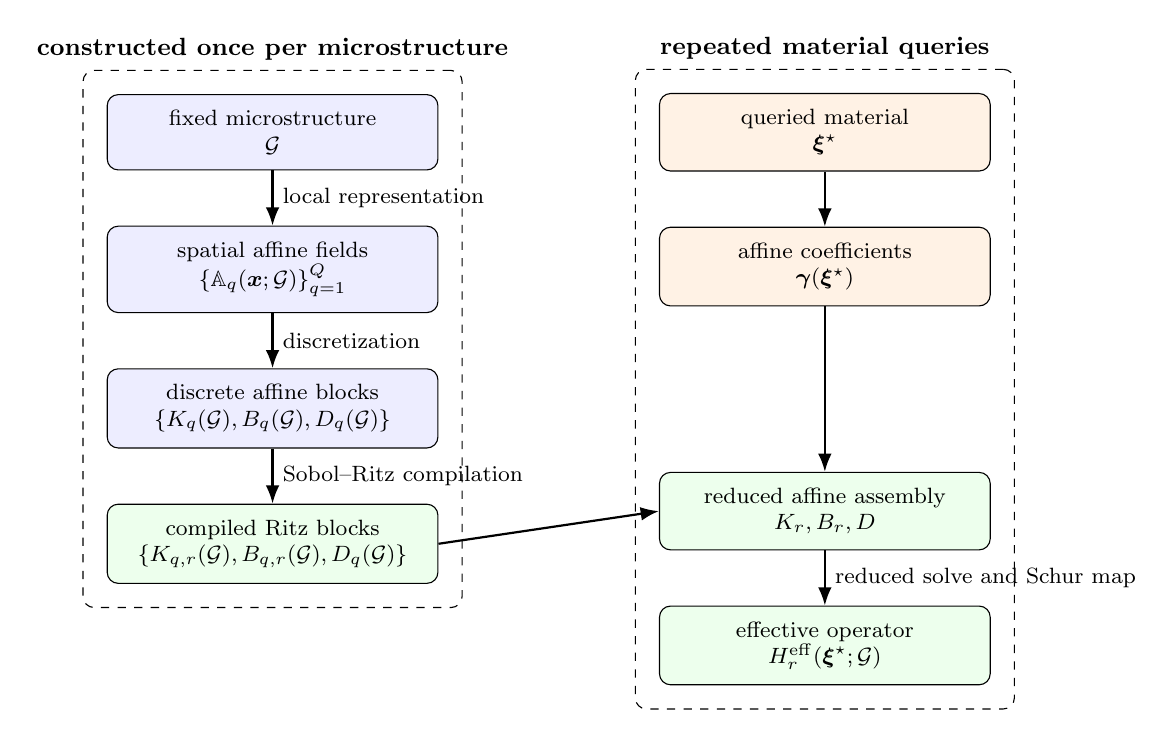
\begin{tikzpicture}[
  >=Latex,
  font=\footnotesize,
  box/.style={draw,rounded corners,align=center,minimum height=8mm,
    text width=38mm,inner sep=2mm},
  geom/.style={box,fill=blue!7},
  mat/.style={box,fill=orange!10},
  op/.style={box,fill=green!7},
  arr/.style={->,thick}
]
\node[geom] (G) {fixed microstructure\\\(\G\)};
\node[geom,below=7mm of G] (A) {spatial affine fields\\\(\{\mathbb A_q(\boldsymbol x;\G)\}_{q=1}^{Q}\)};
\node[geom,below=7mm of A] (F) {discrete affine blocks\\\(\{K_q(\G),B_q(\G),D_q(\G)\}\)};
\node[op,below=7mm of F] (R) {compiled Ritz blocks\\\(\{K_{q,r}(\G),B_{q,r}(\G),D_q(\G)\}\)};

\node[mat,right=28mm of G] (xi) {queried material\\\(\boldsymbol\xi^\star\)};
\node[mat,below=7mm of xi] (gam) {affine coefficients\\\(\boldsymbol\gamma(\boldsymbol\xi^\star)\)};
\node[op,below=21mm of gam] (ass) {reduced affine assembly\\\(K_r,B_r,D\)};
\node[op,below=7mm of ass] (H) {effective operator\\\(\Hr(\boldsymbol\xi^\star;\G)\)};

\draw[arr] (G) -- node[right]{local representation} (A);
\draw[arr] (A) -- node[right]{discretization} (F);
\draw[arr] (F) -- node[right]{Sobol--Ritz compilation} (R);
\draw[arr] (xi) -- (gam);
\draw[arr] (R.east) -- (ass.west);
\draw[arr] (gam) -- (ass);
\draw[arr] (ass) -- node[right]{reduced solve and Schur map} (H);

\node[draw,dashed,rounded corners,fit=(G)(A)(F)(R),inner sep=3mm,
  label={[font=\small\bfseries]above:constructed once per microstructure}] {};
\node[draw,dashed,rounded corners,fit=(xi)(gam)(ass)(H),inner sep=3mm,
  label={[font=\small\bfseries]above:repeated material queries}] {};
\end{tikzpicture}}
\caption{Geometry--material separation across the local, discrete, and
compiled reduced levels. The fixed microstructure determines the spatial
fields and their reusable operators, while each queried material contributes
only the scalar affine coefficients required to assemble and evaluate the
online Ritz--Schur map.}
\label{fig:geometry_material_decoupling}
\end{figure}

\section{Affine compilation of reduced elastic operators}
\label{sec:transfer}

The affine decomposition in Eq.~\eqref{eq:affine_operators} separates the
material dependence, carried by the coefficients
\(\gamma_q(\boldsymbol\xi)\), from the fixed microstructure-dependent blocks
\(K_q(\G)\), \(B_q(\G)\), and \(D_q(\G)\). Consequently, the matrices
\(K(\boldsymbol\xi;\G)\), \(B(\boldsymbol\xi;\G)\), and
\(D(\boldsymbol\xi;\G)\) can be assembled for a new material without
recomputing the spatial contributions of the microstructure. However, the
full-order response in Eq.~\eqref{eq:fom_response} still requires solving the
\(n\)-dimensional system
\(K(\boldsymbol\xi;\G)X(\boldsymbol\xi;\G)=B(\boldsymbol\xi;\G)\)
for every new material.

To remove this remaining material-by-material full-order solve, the proposed
Sobol--Ritz construction samples a limited number of representative materials
through a Sobol sequence and uses their full-order microscopic responses to
define a lower-dimensional Ritz space with \(r\ll n\). Subsequent material
responses are then sought in this space by solving the same discrete
minimum-energy problem of Eq.~\eqref{eq:discrete_energy}, but in reduced
coordinates. This leads naturally to an offline--online formulation: the
microstructure-dependent reduced representation is constructed once during
the offline stage, while each new material is evaluated online using only its
affine coefficients and the precomputed reduced operators. The complete
construction and query paths are previewed in
Fig.~\ref{fig:offline_online_workflow}, before their individual steps are developed
in the following subsections.


\begin{center}
\begin{minipage}{\textwidth}
\captionsetup{hypcap=false,font={sf,small},
  labelfont={bf},labelsep=space,position=top}
\centering
\resizebox{0.98\linewidth}{!}{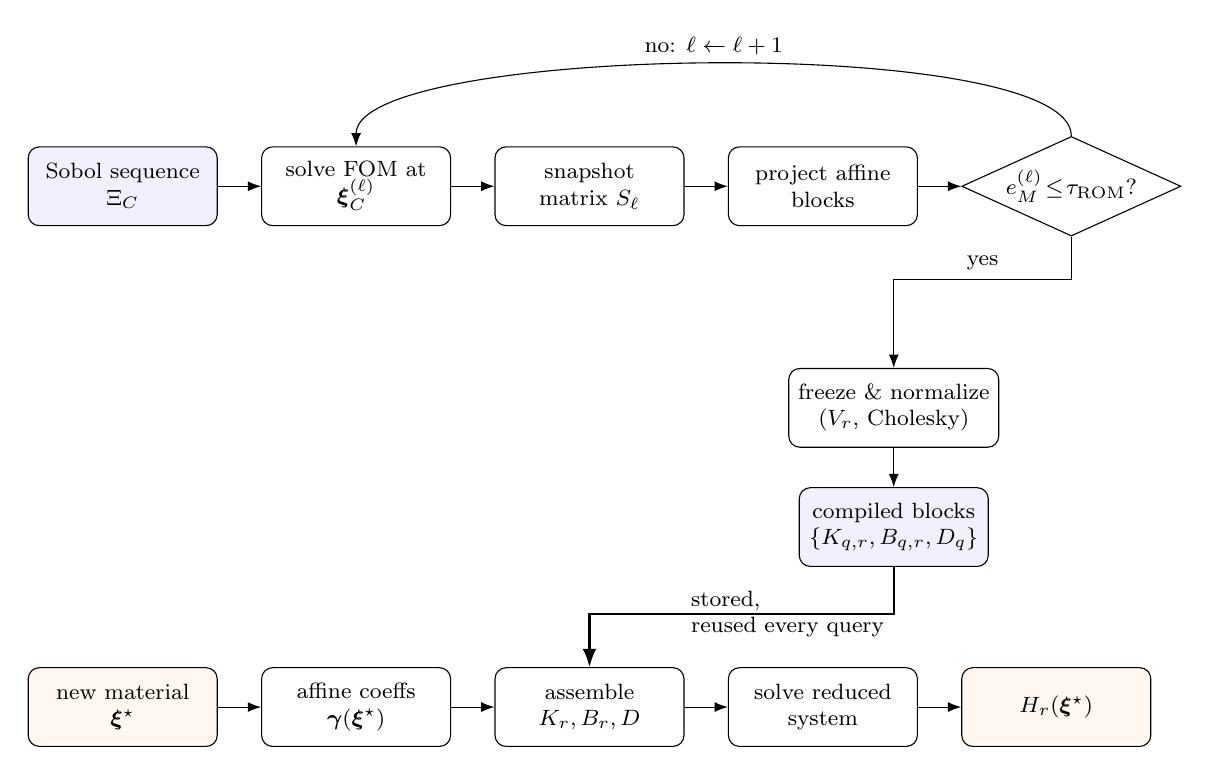
\begin{tikzpicture}[
  >=Latex, font=\footnotesize,
  box/.style={draw, rounded corners, minimum width=2.4cm, minimum height=1.0cm, align=center},
  dec/.style={draw, diamond, aspect=2.2, align=center, inner sep=1pt},
  node distance=0.5cm and 0.55cm
]

% ---------- OFFLINE LANE ----------
\node[box, fill=blue!6] (n1) {Sobol sequence\\$\Xi_C$};
\node[box, right=of n1] (n2) {solve FOM at\\$\boldsymbol\xi_C^{(\ell)}$};
\node[box, right=of n2] (n3) {snapshot\\matrix $S_\ell$};
\node[box, right=of n3] (n4) {project affine\\blocks};
\node[dec, right=of n4] (n5) {$e_M^{(\ell)}\!\le\!\tau_{\mathrm{ROM}}$?};
\node[box, below=1.8cm of n4, xshift=0.9cm] (n6) {freeze \& normalize\\($V_r$, Cholesky)};
\node[box, below=of n6, fill=blue!6] (n7) {compiled blocks\\$\{K_{q,r},B_{q,r},D_q\}$};

\draw[->] (n1) -- (n2);
\draw[->] (n2) -- (n3);
\draw[->] (n3) -- (n4);
\draw[->] (n4) -- (n5);
\draw[->] (n5.south) -- ++(0,-0.55) -| node[pos=0.25,above]{yes} (n6.north);
\draw[->] (n5.north) .. controls +(0,1.3) and +(0,1.3) .. (n2.north)
   node[midway, above]{no: $\ell\leftarrow\ell+1$};
\draw[->] (n6) -- (n7);

% ---------- ONLINE LANE ----------
\node[box, below=5.6cm of n1, fill=orange!6] (m1) {new material\\$\boldsymbol\xi^\star$};
\node[box, right=of m1] (m2) {affine coeffs\\$\boldsymbol\gamma(\boldsymbol\xi^\star)$};
\node[box, right=of m2] (m3) {assemble\\$K_r,B_r,D$};
\node[box, right=of m3] (m4) {solve reduced\\system};
\node[box, right=of m4, fill=orange!6] (m5) {$H_r(\boldsymbol\xi^\star)$};

\draw[->] (m1) -- (m2);
\draw[->] (m2) -- (m3);
\draw[->] (m3) -- (m4);
\draw[->] (m4) -- (m5);

\draw[->, thick] (n7.south) -- ++(0,-0.6) -| node[pos=0.35,right,align=left]{stored,\\reused every query} (m3.north);

\end{tikzpicture}}
\captionof{figure}{Offline compilation and online query stages of the
Sobol--Ritz transfer operator. The offline stage (top) enriches the Ritz
space adaptively until the monitor criterion of
Eq.~\eqref{eq:monitor_stopping} is met, then freezes and normalizes it into
reusable blocks; the online stage (bottom) evaluates any new material at
reduced cost using only those stored blocks. Compare with
Algorithm~\ref{alg:offline_online} for the full pseudocode}
\label{fig:offline_online_workflow}
\end{minipage}
\end{center}

\subsection{Offline construction}
\label{subsec:offline}

The offline stage converts the fixed microstructure \(\G\) into a reusable
set of reduced operators. Full-order responses at selected Sobol materials
define the microscopic response space, which is enriched until the independent
monitor criterion is satisfied and then frozen, normalized in a representative
energy metric, and transformed into the reduced affine blocks used by the
online model.

\subsubsection{Sobol sampling and microscopic response space}
\label{subsubsec:sobol_space}

The microscopic response space is constructed from full-order solutions
evaluated at representative material points within the admissible domain
\(\Xi\), which are selected using a Sobol sequence, a deterministic
low-discrepancy sequence designed to distribute successive samples throughout
a multidimensional domain with limited clustering. Let
\(\Xi_C=\{\boldsymbol\xi_C^{(1)},\ldots,
\boldsymbol\xi_C^{(N_C)}\}\subset\Xi\) denote the resulting fixed candidate
sequence of \(N_C\) material points in their prescribed Sobol order, from
which the training set is taken as the prefix
\(\Xi_S=\{\boldsymbol\xi_C^{(1)},\ldots,
\boldsymbol\xi_C^{(N_s)}\}\). This prefix structure allows additional
materials to be appended without changing those already selected, so the
response space can be enriched sequentially until the adaptive monitoring
procedure introduced in Section~\ref{subsubsec:adaptive_training} determines
the final prefix length \(N_s\).

For each training material
\(\boldsymbol\xi_C^{(j)}\in\Xi_S\), the full-order response system in
Eq.~\eqref{eq:fom_response} is solved for the \(m\) independent macroscopic
loading states, and the resulting microscopic responses are collected in the
snapshot matrix defined in Eq.~\eqref{eq:snapshot_matrix} as
\begin{equation}
\label{eq:snapshot_matrix}
S_{\mathrm{raw}}
=
\left[
X(\boldsymbol\xi_C^{(1)};\G),\ldots,
X(\boldsymbol\xi_C^{(N_s)};\G)
\right]
\in\R^{n\times p},
\qquad
p=mN_s.
\end{equation}

Each column of \(S_{\mathrm{raw}}\) is called a snapshot and contains the
\(n\) coefficients of one full-order microscopic equilibrium response
associated with a particular material and unit macroscopic loading, while
their linear combinations form the sampled microscopic response space
\(\operatorname{range}(S_{\mathrm{raw}})\). The matrix is referred to as raw
because these responses are still expressed in their original full-order
coordinates, before the reference-energy normalization introduced later.
Although \(p=mN_s\) snapshots are collected, some may in principle be exact
linear combinations of others, so the actual dimension of the response space
is given by the rank of \(S_{\mathrm{raw}}\), denoted by \(r\) and defined in
Eq.~\eqref{eq:full_snapshot_rank} as
\begin{equation}
\label{eq:full_snapshot_rank}
r
=
\operatorname{rank}(S_{\mathrm{raw}})
\leq p.
\end{equation}
In the exact-arithmetic full-span construction, the complete response span is retained, so \(r\) is used only to remove exact
linear redundancy rather than to truncate independent microscopic response
directions. Accordingly, if dependent snapshots are present,
\(S\in\R^{n\times r}\) denotes a full-column-rank representation of the same
space, satisfying
\(\operatorname{range}(S)=\operatorname{range}(S_{\mathrm{raw}})\); in the
reported main campaign all snapshot columns are retained, giving \(r=p\) and \(S=S_{\mathrm{raw}}\), while the retained response
dimension remains much smaller than the full microscopic dimension,
\(r\ll n\).

\subsubsection{Ritz projection onto the microscopic response space}
\label{subsubsec:ritz_projection}

In the full-order formulation, the microscopic equilibrium for each material
is obtained from the \(n\)-dimensional system in
Eq.~\eqref{eq:fom_response}, so repeating this solve for every new material
would retain the main computational cost identified in
Section~\ref{sec:transfer}. The snapshot construction in
Section~\ref{subsubsec:sobol_space} provides instead a smaller space
containing the independent microscopic response directions observed over the
training materials, allowing subsequent equilibria to be sought within
\(\operatorname{range}(S)\) rather than over the complete microscopic space.
Using the full-column-rank matrix \(S\in\R^{n\times r}\), the reduced
fluctuation is represented as \(u_r=S\boldsymbol\alpha\), where
\(\boldsymbol\alpha=[\alpha_1,\ldots,\alpha_r]^T\in\R^r\) contains the
coordinates that determine how the retained response directions are combined,
so the equilibrium calculation is reduced from determining \(n\) microscopic
coefficients to determining only \(r\ll n\) reduced coordinates, while the
underlying physical equilibrium problem remains unchanged.

The appropriate coordinates \(\boldsymbol\alpha\) are obtained by preserving
the same minimum-energy principle as the FOM, but restricting the admissible
response to \(\operatorname{range}(S)\), that is,
\(\boldsymbol\alpha=
\operatorname*{arg\,min}_{\boldsymbol\alpha\in\R^r}
\mathcal E(S\boldsymbol\alpha,g;\boldsymbol\xi,\G)\). Substituting
\(u_r=S\boldsymbol\alpha\) into the discrete energy of
Eq.~\eqref{eq:discrete_energy} gives
\(\mathcal E(S\boldsymbol\alpha,g;\boldsymbol\xi,\G)
=\frac{1}{2}\boldsymbol\alpha^TS^TK(\boldsymbol\xi;\G)S\boldsymbol\alpha
-\boldsymbol\alpha^TS^TB(\boldsymbol\xi;\G)g
+\frac{1}{2}g^TD(\boldsymbol\xi;\G)g\), and, since the macroscopic loading
\(g\) is prescribed, stationarity with respect to
\(\boldsymbol\alpha\) leads to the reduced equilibrium system
\begin{equation}
\label{eq:ritz_coordinate_system}
S^T K(\boldsymbol\xi;\G)S\boldsymbol\alpha
=
S^T B(\boldsymbol\xi;\G)g.
\end{equation}
This restricted minimum-energy solution defines the Ritz approximation, with
\(S^TK(\boldsymbol\xi;\G)S\in\R^{r\times r}\) replacing the original
\(n\times n\) microscopic operator, so the same equilibrium principle is
retained while the number of unknowns is reduced from \(n\) to \(r\).

The same reduced equilibrium can be understood through the Galerkin
condition, which provides an equivalent interpretation of
Eq.~\eqref{eq:ritz_coordinate_system}. For the prescribed loading \(g\), the
full-order relation is
\(K(\boldsymbol\xi;\G)u=B(\boldsymbol\xi;\G)g\), whereas the restricted
response \(u_r=S\boldsymbol\alpha\) generally does not satisfy this equation
exactly and therefore leaves the residual
\(r_u=B(\boldsymbol\xi;\G)g-
K(\boldsymbol\xi;\G)S\boldsymbol\alpha\), which measures the remaining
equilibrium imbalance. Requiring \(S^Tr_u=0\) makes this residual orthogonal
to every direction contained in the snapshot space and recovers
Eq.~\eqref{eq:ritz_coordinate_system}; since
\(K(\boldsymbol\xi;\G)\) is symmetric positive definite, the Ritz
minimum-energy condition and the Galerkin orthogonality condition are
therefore equivalent descriptions of the same reduced equilibrium. Moreover,
because every training response
\(X(\boldsymbol\xi_C^{(j)};\G)\) used to construct the snapshot matrix in
Eq.~\eqref{eq:snapshot_matrix} already belongs to
\(\operatorname{range}(S)\), the corresponding FOM solution remains
available within the Ritz space and is reproduced exactly in exact
arithmetic, while approximation is required only for material points whose
full-order responses are not already contained in that space.

Since the microscopic equilibrium is now sought entirely within
\(\operatorname{range}(S)\), the affine operators that govern this equilibrium
must also be expressed in the same reduced space to avoid returning to the
full \(n\)-dimensional formulation during subsequent material evaluations.
Accordingly, the blocks introduced in Eq.~\eqref{eq:affine_operators} are
projected onto \(\operatorname{range}(S)\). Since \(K_q(\G)\) acts on the
microscopic degrees of freedom and \(B_q(\G)\) couples them with the
macroscopic loading, their projected forms are defined in
Eq.~\eqref{eq:raw_affine_blocks} as
\begin{equation}
\label{eq:raw_affine_blocks}
\widetilde K_q
=
S^T K_q(\G)S
\in\R^{r\times r},
\qquad
\widetilde B_q
=
S^T B_q(\G)
\in\R^{r\times m},
\qquad
q=1,\ldots,Q.
\end{equation}
These projected blocks retain the contribution of each affine term within the
microscopic response space, while the tilde indicates that they are still
expressed in the original snapshot coordinates before the reference-energy
normalization introduced in
Section~\ref{subsubsec:reference_energy}; no corresponding projection is
required for \(D_q(\G)\in\R^{m\times m}\), because this block already acts
entirely on the macroscopic loading space.

For clarity, the implementation stores the positive cross-energy contraction
\(\mathcal B_q=-B_q\).
Here \(\overline Z\) contains the \(m\) unit macroscopic driving fields.
The positive coupling is \(\mathcal B_q=|\Omega|^{-1}\int_{\Omega}
(\mathcal L\phi)^T\mathbb A_q\overline Z\,\mathrm d\boldsymbol x\),
and consequently solves
\(\widetilde K(\boldsymbol\xi)\widehat X
=-\widetilde{\mathcal B}(\boldsymbol\xi)\) and evaluates
\(H^{\mathrm{eff}}=D-\widetilde{\mathcal B}^{T}
\widetilde K^{-1}\widetilde{\mathcal B}\). This is algebraically identical
to the sign convention \(B_q=-\mathcal B_q\) used in the variational
definition above; the distinction prevents an ambiguity when reproducing the
voxel contractions from the code.

\subsubsection{Direct voxel-to-reduced compilation}
\label{subsubsec:direct_voxel_compilation}

The definitions above also give a direct implementation route. Let
\(s_j\) be a snapshot column and define its stored microscopic field by
\(z_j=\mathcal Ls_j\). For a prefix \(S_\ell\), collect these fields as
\(Z_\ell(\boldsymbol x)=[z_1(\boldsymbol x),\ldots,z_{r_\ell}(\boldsymbol x)]\).
Let \(\overline Z(\boldsymbol x)\) collect the local macroscopic driving
fields for the \(m\) unit loadings, so that
\(\overline{\boldsymbol z}(\boldsymbol x;g)=\overline Z(\boldsymbol x)g\).
The projected affine blocks can then be evaluated without forming either
global microscopic matrix \(K_q\) or \(B_q\):
\begin{align}
\widetilde K_q^{(\ell)}
&=\frac{1}{|\Omega|}\int_\Omega
Z_\ell(\boldsymbol x)^T\mathbb A_q(\boldsymbol x;\G)
Z_\ell(\boldsymbol x)\,\mathrm d\boldsymbol x,\\
\widetilde{\mathcal B}_q^{(\ell)}
&=\frac{1}{|\Omega|}\int_\Omega
Z_\ell(\boldsymbol x)^T\mathbb A_q(\boldsymbol x;\G)
\overline Z(\boldsymbol x)\,\mathrm d\boldsymbol x,\\
D_q
&=\frac{1}{|\Omega|}\int_\Omega
\overline Z(\boldsymbol x)^T\mathbb A_q(\boldsymbol x;\G)
\overline Z(\boldsymbol x)\,\mathrm d\boldsymbol x.
\end{align}
For the voxel grid these integrals are means over the ordered voxel set. In
the implementation the snapshots already contain the six strain components,
so applying \(\mathcal L\) is part of the FOM snapshot generation rather than
an additional compilation pass. This is a computational reorganization of the
same Galerkin blocks, not a different reduced model.

The constitutive factors are applied on their phase/orientation support. If
\(\mathbb A_{q,v}=U_{q,v}\operatorname{diag}(w_q)U_{q,v}^T\), the contraction
uses \(U_{q,v}^TZ_\ell(\boldsymbol x_v)\) and the corresponding weighted
products. The entries of \(w_q\) retain their signs: individual affine terms can be
indefinite even though their admissible constitutive sum is positive definite.
No positive-definite factorization of each separate term is assumed.
The orientation factors and support ordering are cached once per
geometry; snapshot features are streamed in bounded blocks to keep the GPU
workspace within its memory budget.

When a new block \(\Delta Z_\ell\) is appended, the old--old block is retained
and only the cross and new blocks are computed:
\begin{equation}
\widetilde K_q^{(\ell+1)}=
\begin{bmatrix}
\widetilde K_q^{(\ell)} & C_q^{(\ell)}\\
C_q^{(\ell)T} & \Delta K_q^{(\ell)}
\end{bmatrix},
\qquad
\widetilde{\mathcal B}_q^{(\ell+1)}=
\begin{bmatrix}
\widetilde{\mathcal B}_q^{(\ell)}\\
\Delta\mathcal B_q^{(\ell)}
\end{bmatrix}.
\end{equation}
Here \(C_q^{(\ell)}=|\Omega|^{-1}\int_\Omega
Z_\ell^T\mathbb A_q\Delta Z_\ell\,\mathrm d\boldsymbol x\), while
\(\Delta K_q^{(\ell)}\) and \(\Delta\mathcal B_q^{(\ell)}\) use
\(\Delta Z_\ell\) in the corresponding new--new and macro contractions.
With fixed constitutive ranks and six strain components, this gives an
\(O(N_{\mathrm{vox}}r^2)\) cumulative contraction cost for an enriched
prefix, whereas reassembling every prefix costs
\(O(N_{\mathrm{vox}}\sum_\ell r_\ell^2)\). These estimates describe only
the operator-contraction stage; the FFT snapshot and monitor solves remain
separate terms in the offline budget. Both paths in the controlled benchmark
use incremental updates; their measured difference therefore cannot be
attributed to incremental assembly alone.

The same projection is applied to each intermediate response space generated
during sequential Sobol enrichment, as described in
Section~\ref{subsubsec:adaptive_training}.

\subsubsection{Adaptive enrichment and monitoring}
\label{subsubsec:adaptive_training}

The Sobol sequence fixes the order in which training materials are introduced,
but it does not determine how many are needed, so the response space is
enlarged sequentially until its accuracy is considered sufficient. At
enrichment step \(\ell\), the first \(\ell\) Sobol materials define the
full-column-rank response space
\(S_\ell\in\R^{n\times r_\ell}\), with \(r_\ell\leq m\ell\), and applying the
projection of Eq.~\eqref{eq:raw_affine_blocks} gives the intermediate blocks
\(\widetilde K_q^{(\ell)}=S_\ell^TK_q(\G)S_\ell\) and
\(\widetilde B_q^{(\ell)}=S_\ell^TB_q(\G)\). Each added material can therefore
introduce new microscopic response directions and update the current Ritz
model without removing those already collected, while its accuracy is checked
using an independent monitor set
\(\Xi_M=\{\boldsymbol\xi_M^{(1)},\ldots,
\boldsymbol\xi_M^{(N_M)}\}\subset\Xi\). Training and monitoring thus have
different roles: the Sobol materials construct the response space, whereas
the monitor materials only assess the current approximation and never
contribute snapshots.

Each monitor material is solved once with the FOM to obtain the reference
operator \(\Hfom(\boldsymbol\xi_M^{(j)};\G)\), which is then reused throughout
the enrichment process. For a given step \(\ell\), its affine coefficients
are combined with the current projected blocks to form
\(\widetilde K_\ell(\boldsymbol\xi_M^{(j)};\G)
=\sum_{q=1}^{Q}\gamma_q(\boldsymbol\xi_M^{(j)})
\widetilde K_q^{(\ell)}\) and
\(\widetilde B_\ell(\boldsymbol\xi_M^{(j)};\G)
=\sum_{q=1}^{Q}\gamma_q(\boldsymbol\xi_M^{(j)})
\widetilde B_q^{(\ell)}\), after which the coordinates of the \(m\)
microscopic unit-loading responses,
\(\widehat X_\ell^{(j)}\in\R^{r_\ell\times m}\), are obtained from
\(\widetilde K_\ell\widehat X_\ell^{(j)}=\widetilde B_\ell\). The current
effective operator then follows from the same Schur structure as the FOM,
\(H_\ell^{\mathrm{eff}}
=D-\widetilde B_\ell^T\widehat X_\ell^{(j)}\), so, after the reference FOM
solution has been computed once, subsequent monitor evaluations require only
the current reduced system.

Since the objective of the reduced model is the effective operator itself,
the quality of the current response space is assessed directly from this
quantity using the Frobenius norm
\(\|A\|_F=(\sum_{a,b}A_{ab}^2)^{1/2}\), which combines the differences of all
matrix entries into a single magnitude, so the largest relative error over the
monitor set is defined in Eq.~\eqref{eq:monitor_stopping} as
\begin{equation}
\label{eq:monitor_stopping}
e_M^{(\ell)}
=
\max_{j=1,\ldots,N_M}
\frac{
\left\|
H_\ell^{\mathrm{eff}}(\boldsymbol\xi_M^{(j)};\G)
-
\Hfom(\boldsymbol\xi_M^{(j)};\G)
\right\|_F
}{
\left\|
\Hfom(\boldsymbol\xi_M^{(j)};\G)
\right\|_F
}.
\end{equation}
Hence, \(e_M^{(\ell)}\) is the largest relative effective-operator error
observed over the monitor materials for the current Sobol prefix, and,
starting from a prescribed minimum number \(\ell_{\min}\) of training
materials, this quantity is evaluated after each enrichment step while the
prefix is enlarged one material at a time until the error first falls below
the prescribed tolerance \(\tau_{\mathrm{ROM}}\). This first-crossing rule
defines the final training size in Eq.~\eqref{eq:adaptive_stop} as
\begin{equation}
\label{eq:adaptive_stop}
N_s
=
\min
\left\{
\ell\in\{\ell_{\min},\ldots,N_C\}:
e_M^{(\ell)}
\leq
\tau_{\mathrm{ROM}}
\right\}.
\end{equation}
Thus, \(N_s\) is the smallest Sobol prefix satisfying the monitor criterion,
whereas, if none of the \(N_C\) candidate prefixes reaches the prescribed
tolerance, the target is reported as unmet.

The sequential enrichment also preserves an important variational property,
since each new Sobol material may enlarge the response space but cannot remove
any previously retained direction, so the successive spaces satisfy the
nested relation in Eq.~\eqref{eq:fullrank_nested_spaces}:
\begin{equation}
\label{eq:fullrank_nested_spaces}
\operatorname{range}(S_\ell)
\subseteq
\operatorname{range}(S_{\ell+1}).
\end{equation}
Because each Ritz solution minimizes the same discrete energy over its current
space, enlarging that space can only decrease or preserve the minimum energy,
which leads to the effective-operator ordering stated in
Eq.~\eqref{eq:fullrank_monotone_schur}:
\begin{equation}
\label{eq:fullrank_monotone_schur}
\Hfom(\boldsymbol\xi;\G)
\preceq
H_{\ell+1}^{\mathrm{eff}}(\boldsymbol\xi;\G)
\preceq
H_{\ell}^{\mathrm{eff}}(\boldsymbol\xi;\G).
\end{equation}
The ordering in Eq.~\eqref{eq:fullrank_monotone_schur} means that, for any
macroscopic loading \(g\), the energy associated with the Ritz solution
decreases or remains unchanged as the response space is enriched, approaching
the full-order result from above. Thus, each enrichment step can only improve
or preserve the Ritz effective response in exact arithmetic, while the FOM
remains the full-space reference; the complete proof is given in
Appendix~\ref{app:ritz_ordering}. This monotone enrichment is stopped using
the monitor criterion of Eq.~\eqref{eq:monitor_stopping}, which is evaluated
only over the finite set \(\Xi_M\), so \(\tau_{\mathrm{ROM}}\) should be
interpreted as a practical offline stopping tolerance rather than as an error
bound over the entire domain \(\Xi\), with Eq.~\eqref{eq:adaptive_stop}
determining the final training size \(N_s\) and therefore the point at which
the response space is frozen.

\subsubsection{Reference-energy normalization and final operator compilation}
\label{subsubsec:reference_energy}

Once the adaptive procedure in Section~\ref{subsubsec:adaptive_training}
determines \(N_s\), the response space is frozen and no further microscopic
directions are added. Although the resulting matrix \(S\) already spans the
desired Ritz space, its columns come from different materials and loading
states and may therefore have different energetic scales or be closely
related, which can lead to poorly scaled reduced matrices. The response space
is therefore re-expressed in a reference-energy coordinate system that
improves its numerical scaling without changing its dimension or removing any
of the retained information.

A representative microscopic operator is first constructed from the complete
Sobol candidate sequence by averaging its affine coefficient vectors. The
average coefficients and the corresponding reference operator are defined in
Eq.~\eqref{eq:reference_energy_operator} as
\begin{equation}
\label{eq:reference_energy_operator}
\overline{\boldsymbol\gamma}
=
\frac{1}{N_C}
\sum_{j=1}^{N_C}
\boldsymbol\gamma(\boldsymbol\xi_C^{(j)})
\in\R^Q,
\qquad
K_{\mathrm{ref}}(\G)
=
\sum_{q=1}^{Q}
\overline{\gamma}_qK_q(\G)
\in\R^{n\times n}.
\end{equation}
Using the affine representation in Eq.~\eqref{eq:affine_operators},
\(K_{\mathrm{ref}}(\G)\) is simply the average microscopic operator associated
with the candidate materials, so it provides a representative energetic scale
for the admissible material domain. Candidate points outside the selected
training prefix contribute only their affine coefficients to this average,
which requires no additional FOM solutions and introduces no new snapshots.

The reference operator defines the energy-based inner product
\(\langle a,b\rangle_{K_{\mathrm{ref}}}=a^TK_{\mathrm{ref}}b\), which
measures how two retained microscopic directions relate to each other under
this representative energy. Applying it to all pairs of columns of \(S\)
gives the Gram matrix
\(G_{\mathrm{ref}}=S^TK_{\mathrm{ref}}S\), whose entries collect these
pairwise energy products; using
Eqs.~\eqref{eq:reference_energy_operator} and
\eqref{eq:raw_affine_blocks}, this matrix can be assembled directly from the
already projected blocks as
\(G_{\mathrm{ref}}
=\sum_{q=1}^{Q}\overline{\gamma}_q\widetilde K_q\), without returning to the
full-dimensional operators.

Since \(S\) has full column rank and \(K_{\mathrm{ref}}\) is symmetric
positive definite, \(G_{\mathrm{ref}}\) is also positive definite and can be
factorized by Cholesky. This factorization is then used to rescale and
orthogonalize the Ritz coordinates in the reference-energy metric, as defined
in Eq.~\eqref{eq:reference_energy_qr}:
\begin{equation}
\label{eq:reference_energy_qr}
G_{\mathrm{ref}}
=
S^TK_{\mathrm{ref}}S
=
R_{\mathrm{ref}}^TR_{\mathrm{ref}},
\qquad
V_r
=
SR_{\mathrm{ref}}^{-1},
\end{equation}
where \(R_{\mathrm{ref}}\in\R^{r\times r}\) is the invertible
upper-triangular Cholesky factor and
\(V_r\in\R^{n\times r}\) is the resulting reference-energy Ritz basis. From
Eq.~\eqref{eq:reference_energy_qr},
\(V_r^TK_{\mathrm{ref}}V_r=I\), so the columns of \(V_r\) have unit scale and
are mutually orthogonal with respect to the reference energy, while
\(\operatorname{range}(V_r)=\operatorname{range}(S)\) because
\(R_{\mathrm{ref}}\) is invertible. The normalization therefore changes only
the coordinates used to describe the Ritz space and does not truncate or
modify the space itself.

The affine blocks can now be written in these normalized coordinates, so the
operators required for future material queries are stored directly in the
final Ritz basis. Using
\(K_{q,r}=V_r^TK_q(\G)V_r\),
\(B_{q,r}=V_r^TB_q(\G)\), and
\(V_r=SR_{\mathrm{ref}}^{-1}\), together with
Eq.~\eqref{eq:raw_affine_blocks}, gives the compiled blocks in
Eq.~\eqref{eq:raw_ritz_transform}:
\begin{equation}
\label{eq:raw_ritz_transform}
K_{q,r}(\G)
=
R_{\mathrm{ref}}^{-T}
\widetilde K_q
R_{\mathrm{ref}}^{-1}
\in\R^{r\times r},
\qquad
B_{q,r}(\G)
=
R_{\mathrm{ref}}^{-T}
\widetilde B_q
\in\R^{r\times m}.
\end{equation}
Because Eq.~\eqref{eq:raw_ritz_transform} uses only the already projected
blocks, the full-dimensional basis \(V_r\) does not need to be formed
explicitly during compilation. Together with the unchanged macroscopic blocks
\(D_q(\G)\in\R^{m\times m}\), the set
\(\{K_{q,r}(\G),B_{q,r}(\G),D_q(\G)\}_{q=1}^{Q}\) is the final
microstructure-dependent representation stored for the online material
queries introduced in Section~\ref{subsec:reduced_transfer}.

\paragraph{The same compiled blocks in POD coordinates.}
For a fixed positive-definite metric \(W\), let
\(G_W=S^TWS=U\Lambda U^T\). Retaining \(k\) positive modes defines
\(T_k=U_k\Lambda_k^{-1/2}\) and the POD basis \(Q_k=ST_k\).
Its affine blocks are obtained entirely in reduced coordinates:
\begin{equation}
K_q^{\mathrm{POD}}=T_k^T\widetilde K_qT_k,\qquad
B_q^{\mathrm{POD}}=T_k^T\widetilde B_q,\qquad
D_q^{\mathrm{POD}}=D_q.
\label{eq:pod_block_transform}
\end{equation}
For energy POD, \(G_W=G_{\mathrm{ref}}\) is already available. If all modes
are retained, this is an invertible change of coordinates and the effective
Schur output is unchanged in exact arithmetic. Truncation changes the
approximation space; in the comparison below its dimension is selected on
monitors, without inspecting held-out outputs. Neither this equivalence nor
metric reuse requires reconstructing the POD fields on the voxel grid.

\subsection{Online Ritz--Schur transfer}
\label{subsec:reduced_transfer}

After the reference-energy normalization in
Section~\ref{subsubsec:reference_energy}, the fixed microstructure is fully
represented by the compiled blocks
\(\{K_{q,r}(\G),B_{q,r}(\G),D_q(\G)\}_{q=1}^{Q}\), so a new material
\(\boldsymbol\xi^\star\in\Xi\) enters the online model only through its affine
coefficients \(\gamma_q(\boldsymbol\xi^\star)\). These coefficients are used
to combine the stored blocks, giving the material-dependent reduced operators
defined in Eq.~\eqref{eq:online_assembly}:
\begin{equation}
\label{eq:online_assembly}
\begin{aligned}
K_r(\boldsymbol\xi^\star;\G)
&=
\sum_{q=1}^{Q}
\gamma_q(\boldsymbol\xi^\star)K_{q,r}(\G),
\\
B_r(\boldsymbol\xi^\star;\G)
&=
\sum_{q=1}^{Q}
\gamma_q(\boldsymbol\xi^\star)B_{q,r}(\G),
\\
D(\boldsymbol\xi^\star;\G)
&=
\sum_{q=1}^{Q}
\gamma_q(\boldsymbol\xi^\star)D_q(\G).
\end{aligned}
\end{equation}
Here,
\(K_r(\boldsymbol\xi^\star;\G)\in\R^{r\times r}\),
\(B_r(\boldsymbol\xi^\star;\G)\in\R^{r\times m}\), and
\(D(\boldsymbol\xi^\star;\G)\in\R^{m\times m}\), so changing the material
modifies only the scalar weights used to combine the precomputed
microstructure-dependent blocks, without requiring a new spatial assembly or
projection.

The \(m\) microscopic unit-loading responses are then represented in the
normalized Ritz space as
\(X_r=V_r\widehat X_r\), where
\(\widehat X_r\in\R^{r\times m}\) contains their reduced coordinates.
Applying the same Ritz--Galerkin condition introduced in
Section~\ref{subsubsec:ritz_projection} gives the reduced equilibrium system
in Eq.~\eqref{eq:reduced_response}:
\begin{equation}
\label{eq:reduced_response}
K_r(\boldsymbol\xi^\star;\G)
\widehat X_r(\boldsymbol\xi^\star;\G)
=
B_r(\boldsymbol\xi^\star;\G).
\end{equation}
The microscopic equilibrium is therefore obtained from a system of dimension
\(r\) rather than \(n\), with \(r\ll n\), after which the effective operator
follows from the same Schur elimination used by the FOM. Since
\(X_r=V_r\widehat X_r\) and \(B_r=V_r^TB\), the microscopic contribution
\(B^TX_r\) can be evaluated directly as
\(B_r^T\widehat X_r\), leading to the online Ritz--Schur transfer defined in
Eq.~\eqref{eq:reduced_transfer}:
\begin{equation}
\label{eq:reduced_transfer}
\Hr(\boldsymbol\xi^\star;\G)
=
D(\boldsymbol\xi^\star;\G)
-
B_r(\boldsymbol\xi^\star;\G)^T
\widehat X_r(\boldsymbol\xi^\star;\G)
\in\R^{m\times m}.
\end{equation}
Thus, the queried material is mapped directly to its effective constitutive
operator using only reduced quantities, while the full microscopic response
\(X_r=V_r\widehat X_r\) does not need to be reconstructed during the online
evaluation.

For fixed \(m\), assembling the reduced affine operators requires
\(\mathcal O(Qr^2)\) operations and solving
Eq.~\eqref{eq:reduced_response} requires
\(\mathcal O(r^3)\), giving an online complexity of
\(\mathcal O(Qr^2+r^3)\). Although the reduced solve therefore scales
cubically with \(r\), this dimension is much smaller than the full
microscopic dimension, \(r\ll n\), so the resulting dense algebra remains
inexpensive. By comparison, the Fourier--Galerkin FOM used in the numerical
assessment requires approximately
\(\mathcal O(mI_{\mathrm{CG}}N_{\mathrm{vox}}\log N_{\mathrm{vox}})\) per
material, where \(I_{\mathrm{CG}}\) is the representative number of
conjugate-gradient iterations and \(N_{\mathrm{vox}}\) is the total number
of voxels. In the three-dimensional strain-based implementation, the FOM
stores six microscopic field components per voxel and therefore operates on
an ambient representation of size \(6N_{\mathrm{vox}}\), while \(n\) denotes
the number of independent unknowns after the discrete admissibility constraints
are imposed. Consequently, \(n\) scales linearly with
\(N_{\mathrm{vox}}\), and the online cost is governed by the small Ritz
dimension \(r\ll n\) rather than by the spatial resolution of the
microstructure. The resulting reduction
in query time is quantified for the three-dimensional elasticity cases in
Section~\ref{subsec:computational_performance}.

\subsection{Ritz--Schur error identity}
\label{subsec:ritz_schur_identity}

The Ritz construction also provides an exact relation between the microscopic
response error and the resulting difference in the effective operator. For a
fixed material--microstructure pair \((\boldsymbol\xi,\G)\), let
\(\Delta X=X-X_r\in\R^{n\times m}\) denote the difference between the FOM and
ROM microscopic responses, and let \(R=B-KX_r\in\R^{n\times m}\) denote the
residual obtained when the ROM response is inserted into the full-order
equilibrium equation. A vanishing residual, \(R=0\), means that the ROM
satisfies the FOM equilibrium exactly, whereas \(R\neq0\) indicates that some
microscopic equilibrium error remains; this connection follows directly from
the FOM relation \(KX=B\) and the definition
\(X=X_r+\Delta X\), which give
\(R=B-KX_r=KX-KX_r=K\Delta X\). Since
\(K(\boldsymbol\xi;\G)\) is invertible, \(R=0\) is therefore equivalent to
\(\Delta X=0\), showing that the residual directly measures the remaining
difference between the FOM and ROM microscopic responses.

Combining this relation with the Galerkin orthogonality established in
Section~\ref{subsubsec:ritz_projection} gives the exact Ritz--Schur identity
in Eq.~\eqref{eq:ritz_schur_identity}:
\begin{equation}
\label{eq:ritz_schur_identity}
\Hr(\boldsymbol\xi;\G)
-
\Hfom(\boldsymbol\xi;\G)
=
(\Delta X)^T
K(\boldsymbol\xi;\G)
(\Delta X)
=
R^T
K(\boldsymbol\xi;\G)^{-1}
R
\succeq0.
\end{equation}
The complete algebraic derivation is provided in
Appendix~\ref{app:ritz_schur_identity_derivation}. The condition
\(\succeq0\) means that the difference between the reduced and full-order
operators gives a nonnegative energy for every macroscopic loading \(g\),
since
\(g^T[\Hr-\Hfom]g
=(\Delta Xg)^TK(\Delta Xg)\geq0\). Thus, the effective-operator difference is
exactly the microscopic Ritz error measured through the energy associated
with \(K\), which is consistent with the Loewner ordering introduced in
Section~\ref{subsubsec:adaptive_training}.

Equation~\eqref{eq:ritz_schur_identity} is exact with respect to the discrete
FOM, but evaluating the term \(R^TK^{-1}R\) directly would require applying
the full-order inverse and would therefore remove the main advantage of the
online model. The identity is consequently used here to establish the
variational relation between the Ritz and FOM operators rather than as an
online error estimator, while the accuracy of the frozen reduced model is
assessed independently on material points that played no role in its
construction.

\paragraph{Finite precision and coordinate conditioning.}
The variational identity is an exact-arithmetic result. Nearly dependent
snapshots and cancellation between signed affine terms can amplify errors in
float32 volumetric contractions. Re-expressing reduced coordinates in an
energy metric, or equilibrating a reduced system by a diagonal congruence,
can improve its scaling but cannot recover accuracy already lost during
contraction. For example, with \(P_{ii}=\sqrt{(K_r)_{ii}}\), the system
\(P^{-1}K_rP^{-1}y=P^{-1}B_r\) is algebraically equivalent to the original
system, with \(\widehat X=P^{-1}y\). This requires no voxel pass, but its
runtime overhead and numerical benefit must be measured separately. It is
not a finite-precision positivity certificate. The timing campaign below
refers to the archived solver configuration used in that campaign; subsequent
conditioning changes are not credited with those timings. Negative numerical
Schur gaps are reported explicitly, rather than removed from the validation
statistics or interpreted as a disproof of the exact identity.

\subsection{Independent held-out validation}
\label{subsec:heldout_validation}

The monitor set \(\Xi_M\) cannot be used as the final accuracy test because it
already participates in the offline construction by determining where the
Sobol enrichment is stopped, so, after \(N_s\), the response space, and the
compiled operators have been frozen, a separate held-out set
\(\Xi_V=\{\boldsymbol\xi_V^{(1)},\ldots,
\boldsymbol\xi_V^{(N_V)}\}\subset\Xi\) is evaluated with both the FOM and the
completed Ritz model. For each held-out material, the relative
effective-operator error is defined in Eq.~\eqref{eq:validation_error} as
\begin{equation}
\label{eq:validation_error}
e_{V,j}
=
\frac{
\left\|
\Hr(\boldsymbol\xi_V^{(j)};\G)
-
\Hfom(\boldsymbol\xi_V^{(j)};\G)
\right\|_F
}{
\left\|
\Hfom(\boldsymbol\xi_V^{(j)};\G)
\right\|_F
},
\qquad
j=1,\ldots,N_V.
\end{equation}
These FOM evaluations are performed only after the reduced model has been
completed and therefore cannot change \(N_s\), the Ritz space, the
reference-energy normalization, or any compiled operator. The two material
sets consequently have distinct purposes: \(\Xi_M\) provides the practical
offline stopping criterion, whereas \(\Xi_V\) measures the predictive
accuracy of the final model on previously unseen materials.

\subsection{Offline--online workflow}
\label{subsec:offline_online}

The preceding construction separates the computational work into two stages:
the fixed microstructure is compiled once using full-order information during
the offline stage, whereas each subsequent material query uses only the
stored reduced operators and its affine constitutive coefficients. The complete
sequence is summarized in Algorithm~\ref{alg:offline_online}, while the
held-out evaluation is included separately at the end of the algorithm only
as a post-freeze assessment and does not modify the compiled model.

\begin{algorithm}[H]
\caption{Offline compilation, online query, and independent validation of the
Sobol--Ritz transfer operator for a fixed microstructure \(\G\).}
\label{alg:offline_online}
\small

\textbf{Input:}
fixed microstructure \(\G\), constitutive domain \(\Xi\), Sobol candidate
sequence \(\Xi_C\), monitor set \(\Xi_M\), tolerance
\(\tau_{\mathrm{ROM}}\), and first monitored prefix size
\(\ell_{\min}\).

\textbf{Offline compilation}

\begin{tabbing}
\hspace{0.5cm}\=\hspace{0.7cm}\=\hspace{0.7cm}\=\kill

Prepare phase/orientation factors and macro blocks \(D_q\).
Do not assemble global matrices \(K_q\) or \(B_q\). \\

Evaluate each material in \(\Xi_M\) once with the FOM and store
\(\Hfom(\boldsymbol\xi_M^{(j)};\G)\). \\

Initialize the snapshot collection. \\[1mm]

\textbf{for} \(\ell=1,\ldots,N_C\) \textbf{do} \\

\> Solve Eq.~\eqref{eq:fom_response} at
\(\boldsymbol\xi_C^{(\ell)}\) for the \(m\) unit macroscopic loadings. \\

\> Append
\(X(\boldsymbol\xi_C^{(\ell)};\G)\)
to the accumulated snapshot matrix. \\

\> Form a full-column-rank matrix \(S_\ell\) that preserves the complete
accumulated response span, removing exact redundancies only. \\

\> Contract only new and cross blocks to update
\(\{\widetilde K_q^{(\ell)},
\widetilde B_q^{(\ell)}\}_{q=1}^{Q}\)
from Eq.~\eqref{eq:raw_affine_blocks}. \\[1mm]

\> \textbf{if} \(\ell\geq\ell_{\min}\) \textbf{then} \\

\>\> Evaluate the monitor materials using the current Ritz model. \\

\>\> Compute the maximum monitor error
\(e_M^{(\ell)}\)
from Eq.~\eqref{eq:monitor_stopping}. \\

\>\> \textbf{if}
\(e_M^{(\ell)}\leq\tau_{\mathrm{ROM}}\)
\textbf{then} \\

\>\>\> Set
\(N_s\leftarrow\ell\),
\(S\leftarrow S_\ell\), and
\(r\leftarrow r_\ell\). \\

\>\>\> Freeze
\(\widetilde K_q\leftarrow\widetilde K_q^{(\ell)}\) and
\(\widetilde B_q\leftarrow\widetilde B_q^{(\ell)}\)
for \(q=1,\ldots,Q\). \\

\>\>\> \textbf{break}. \\

\>\> \textbf{end if} \\

\> \textbf{end if} \\

\textbf{end for} \\[1mm]

\textbf{if} no prefix satisfies Eq.~\eqref{eq:adaptive_stop}
\textbf{then} \\

\> Report the prescribed tolerance as unmet and terminate the compilation. \\

\textbf{end if} \\[1mm]

Compute the average affine coefficients
\(\overline{\boldsymbol\gamma}\) and the reference operator
\(K_{\mathrm{ref}}(\G)\)
using Eq.~\eqref{eq:reference_energy_operator}. \\

Assemble
\(G_{\mathrm{ref}}
=\sum_{q=1}^{Q}
\overline{\gamma}_q\widetilde K_q\)
and compute the Cholesky factor
\(R_{\mathrm{ref}}\)
using Eq.~\eqref{eq:reference_energy_qr}. \\

Transform the frozen projected blocks into the normalized operators
\(\{K_{q,r}(\G),B_{q,r}(\G)\}_{q=1}^{Q}\)
using Eq.~\eqref{eq:raw_ritz_transform}. \\

Store
\(\{K_{q,r}(\G),B_{q,r}(\G),D_q(\G)\}_{q=1}^{Q}\)
as the compiled representation of \(\G\).

\end{tabbing}

\textbf{Online material query}

\begin{tabbing}
\hspace{0.5cm}\=\hspace{0.7cm}\=\kill

\textbf{Given}
\(\boldsymbol\xi^\star\in\Xi\): \\

Evaluate its affine coefficients
\(\boldsymbol\gamma(\boldsymbol\xi^\star)\). \\

Assemble
\(K_r(\boldsymbol\xi^\star;\G)\),
\(B_r(\boldsymbol\xi^\star;\G)\), and
\(D(\boldsymbol\xi^\star;\G)\)
using Eq.~\eqref{eq:online_assembly}. \\

Solve Eq.~\eqref{eq:reduced_response} for
\(\widehat X_r(\boldsymbol\xi^\star;\G)\). \\

Evaluate
\(\Hr(\boldsymbol\xi^\star;\G)\)
using Eq.~\eqref{eq:reduced_transfer}. \\

\textbf{return}
\(\Hr(\boldsymbol\xi^\star;\G)\).

\end{tabbing}

\textbf{Independent post-freeze validation}

\begin{tabbing}
\hspace{0.5cm}\=\hspace{0.7cm}\=\kill

\textbf{Given}
\(\Xi_V=\{\boldsymbol\xi_V^{(1)},\ldots,
\boldsymbol\xi_V^{(N_V)}\}\): \\

\textbf{for} \(j=1,\ldots,N_V\) \textbf{do} \\

\> Evaluate
\(\Hfom(\boldsymbol\xi_V^{(j)};\G)\)
with the FOM. \\

\> Evaluate
\(\Hr(\boldsymbol\xi_V^{(j)};\G)\)
with the frozen reduced model. \\

\> Compute \(e_{V,j}\) using
Eq.~\eqref{eq:validation_error}. \\

\textbf{end for}

\end{tabbing}

\end{algorithm}

\section{Numerical assessment in linear elasticity}
\label{sec:numerical_assessment}

The proposed Sobol--Ritz transfer formulation is assessed in
three-dimensional linear elasticity over ten periodic composite
microstructures. Elasticity is selected as a conservative representative case
because it requires six independent macroscopic loading states, providing an
upper workload with respect to the number of load cases among the physical
problems considered here. The assessment then examines adaptive construction,
independent held-out accuracy, computational performance, and comparison with
data-only surrogates.

\subsection{Problem setup and numerical campaign}
\label{subsec:elasticity_setup}

For three-dimensional linear elasticity, the general formulation introduced
in Section~\ref{sec:homogenization} specializes as
\begin{equation}
\label{eq:elastic_specialization}
m=6,
\qquad
\mathcal L u
=
\boldsymbol{\varepsilon}(u),
\qquad
\mathbb A
=
\mathbb C,
\qquad
\Heff
=
\Ceff.
\end{equation}
Equation~\eqref{eq:elastic_specialization} implies
\(X\in\R^{n\times6}\), \(\Hfom=\Cfom\), and \(\Hr=\Cr\). Accordingly, the
full-order Schur map in Eq.~\eqref{eq:schur_transfer} becomes
\(\Cfom=D-B^TK^{-1}B\).

The constitutive family consists of an isotropic matrix and transversely
isotropic fibers. The queried material vector is
\begin{equation}
\label{eq:elastic_material_vector}
\boldsymbol\xi
=
(E_m,\nu_m,E_L,E_T,G_{LT},\nu_{LT},\nu_{TT}).
\end{equation}
The seven quantities in Eq.~\eqref{eq:elastic_material_vector} define the
admissible constitutive domain used throughout the numerical campaign.
For this material family, the affine representation contains \(Q=7\)
coefficients. Their explicit construction in Mandel notation, including the
local fiber-frame rotation, is provided in Appendix~\ref{app:affine}.

The numerical campaign spans both constitutive and geometric variation. The
admissible material domain is defined by the seven constitutive parameters in
Table~\ref{tab:material_domain}, while the ten fixed microstructures G00--G09
in Table~\ref{tab:geometry_campaign} vary in fiber volume fraction, aspect
ratio, and orientation distribution. Each microstructure is compiled
independently into its own Sobol--Ritz operator. Figure~\ref{fig:geometry_slices}
shows representative central voxel slices of the ten cells to illustrate their
geometric variation.

\begin{center}
\begin{minipage}[t]{0.45\textwidth}
\vspace{0pt}
\captionsetup{hypcap=false,font={sf,small},
  labelfont={bf},labelsep=space,position=top}
\centering
\scriptsize
\captionof{table}{Constitutive-parameter domain used in the numerical assessment.}
\label{tab:material_domain}
\resizebox{\linewidth}{!}{%
\begin{tabular}{@{}lcc@{}}
\toprule
Parameter & Symbol & Range \\
\midrule
Matrix Young's modulus & \(E_m\) & \([1.1,4.4]~\si{\giga\pascal}\) \\
Matrix Poisson ratio & \(\nu_m\) & \([0.35,0.42]\) \\
Fiber longitudinal modulus & \(E_L\) & \([72,395]~\si{\giga\pascal}\) \\
Fiber transverse modulus & \(E_T\) & \([6,23]~\si{\giga\pascal}\) \\
Fiber longitudinal shear modulus & \(G_{LT}\) & \([8,30]~\si{\giga\pascal}\) \\
Fiber longitudinal Poisson ratio & \(\nu_{LT}\) & \([0.20,0.26]\) \\
Fiber transverse Poisson ratio & \(\nu_{TT}\) & \([0.35,0.40]\) \\
\bottomrule
\end{tabular}%
}
\end{minipage}
\hfill
\begin{minipage}[t]{0.50\textwidth}
\vspace{0pt}
\captionsetup{hypcap=false,font={sf,small},
  labelfont={bf},labelsep=space,position=top}
\centering
\scriptsize
\captionof{table}{Fixed microstructures used in the numerical campaign.
The volume fraction is measured after voxelization.}
\label{tab:geometry_campaign}
\resizebox{\linewidth}{!}{%
\begin{tabular}{@{}lcccc@{}}
\toprule
Microstructure & \(V_f\) & Aspect ratio & Orientation \((a_{11},a_{22},a_{33})\) & Grid \\
\midrule
G00 & 0.1502 & 12.5 & \((1/3,1/3,1/3)\) & \(150^3\) \\
G01 & 0.0497 & 12.5 & \((1/3,1/3,1/3)\) & \(150^3\) \\
G02 & 0.2502 & 12.5 & \((1/3,1/3,1/3)\) & \(150^3\) \\
G03 & 0.1514 & 5.0 & \((1/3,1/3,1/3)\) & \(60^3\) \\
G04 & 0.1499 & 20.0 & \((1/3,1/3,1/3)\) & \(240^3\) \\
G05 & 0.1483 & 12.5 & \((0.50,0.50,0)\) & \(150^3\) \\
G06 & 0.1502 & 12.5 & \((0.90,0.05,0.05)\) & \(150^3\) \\
G07 & 0.1497 & 12.5 & \((0.65,0.25,0.10)\) & \(150^3\) \\
G08 & 0.0489 & 5.0 & \((1/3,1/3,1/3)\) & \(60^3\) \\
G09 & 0.2498 & 20.0 & \((1/3,1/3,1/3)\) & \(240^3\) \\
\bottomrule
\end{tabular}%
}
\end{minipage}
\end{center}

\begin{center}
\begin{minipage}{\textwidth}
\captionsetup{hypcap=false}
\centering
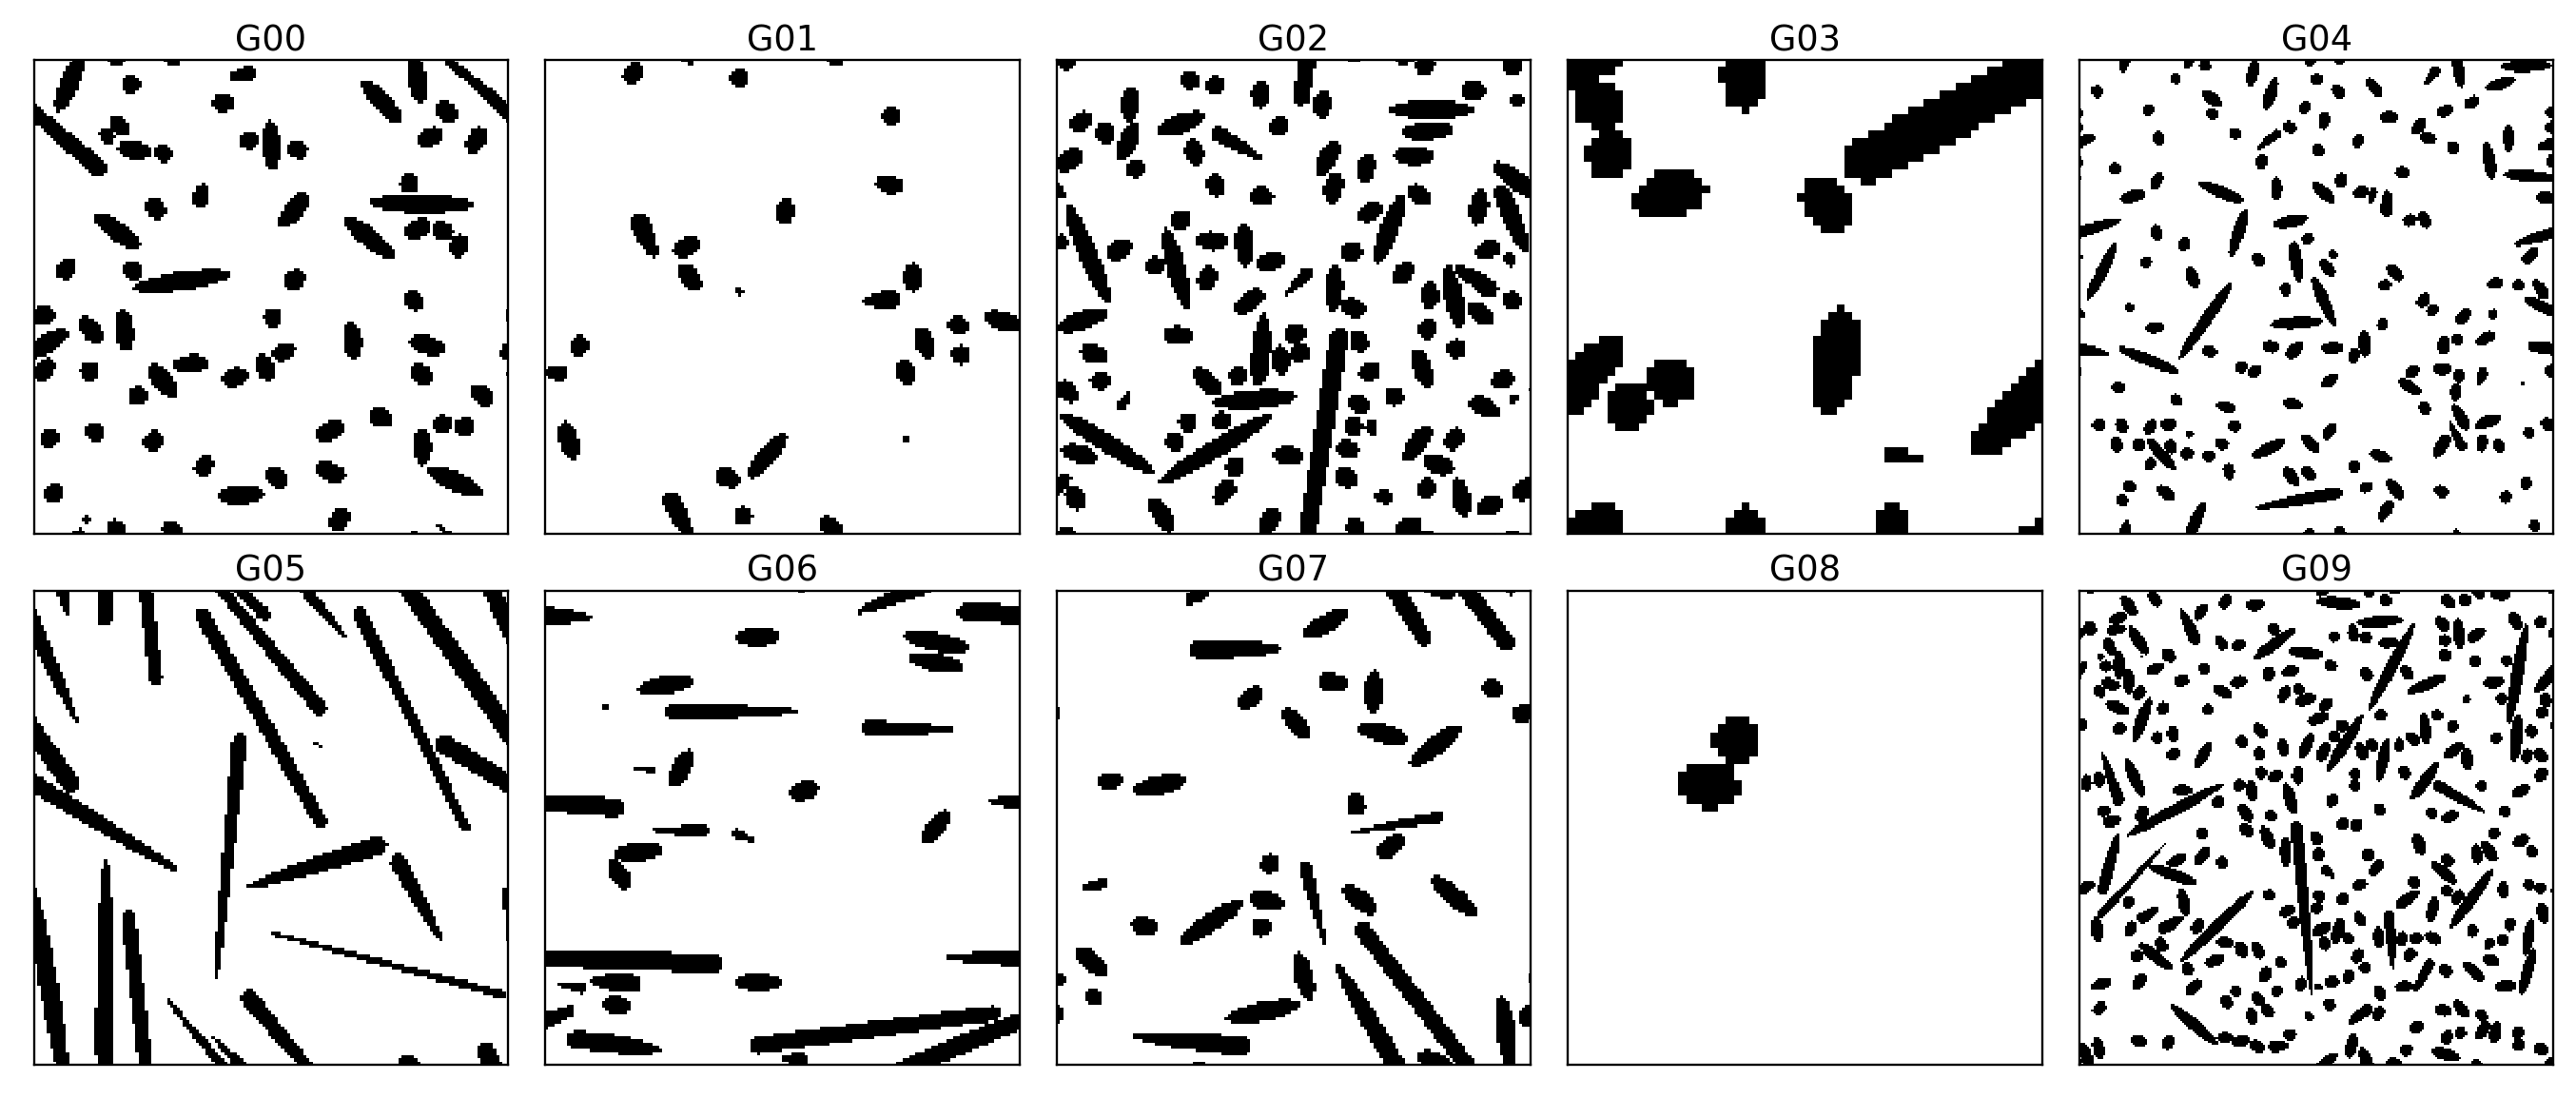
\includegraphics[width=\textwidth]{figures/numerical_geometry_slices.png}
\captionof{figure}{Central slices of the periodic microstructures G00--G09.
Black and white denote the fiber and matrix phases, respectively}
\label{fig:geometry_slices}
\end{minipage}
\end{center}

For each microstructure, a fixed Sobol candidate sequence of \(N_C=1024\)
constitutive points is used. Adaptive enrichment starts from
\(\ell_{\min}=2\) materials and is controlled by an independent monitor set
of \(N_M=5\) materials with
\(\tau_{\mathrm{ROM}}=10^{-4}\). After the reduced model is frozen,
its accuracy is assessed on an independent \(N_V=20\) maximin design selected
from a separate 4096-point Sobol pool. The same material designs are used for
G00--G09. The five monitor materials require additional full-order solves;
therefore 6--16 training materials mean 11--21 construction materials per
geometry, each with six load cases. The 20 validation materials are charged
separately. Sharing the validation design gives 200 material--geometry pairs,
not 200 independently drawn material vectors.

All reported microstructures are discretized using 6 voxels per fiber diameter,
with the resolution-convergence study in Appendix~\ref{app:voxel_resolution}
showing that, for the representative cells G08, G00, and G09, the relative
change in effective stiffness between 5 and 6 voxels per fiber diameter ranges
from \(0.099\%\) to \(0.910\%\). These changes exceed some reported
reduction errors and do not establish convergence to a continuum reference;
ROM accuracy below is measured against the corresponding voxel-discrete FOM.

\subsection{Adaptive construction and independent validation}
\label{subsec:adaptive_results}

\paragraph{Adaptive construction.}
\label{par:adaptive_construction}

Table~\ref{tab:adaptive_accuracy} summarizes the adaptive construction results
for the ten microstructures. The first-crossing criterion selects
\(N_s=6\)--16 training materials, corresponding to final snapshot ranks of
\(r=36\)--96, while all microstructures satisfy the prescribed \(0.01\%\)
monitor threshold. The required reduced-space dimension varies noticeably
across geometries: the dilute cells G01 and G08 satisfy the stopping criterion
with only six training materials, whereas G09 requires 16. This variation
indicates that, even over the same constitutive domain, the complexity of the
transferable microscopic response space depends strongly on the underlying
microstructure.

\begin{table}[t]
\setlength{\tabcolsep}{3.5pt}
\caption{Adaptive construction and independent held-out validation.
Relative errors are reported in percent. Eigenvalues of \(K_r\) are
dimensionless in reference-energy coordinates; those of \(\Cr\) are in
\si{\giga\pascal}.}
\label{tab:adaptive_accuracy}
\begin{tabular}{@{}lrrrrrrr@{}}
\toprule
& \multicolumn{3}{c}{Adaptive construction} &
\multicolumn{2}{c}{Held-out accuracy} &
\multicolumn{2}{c}{Stability diagnostics} \\
\cmidrule(lr){2-4}
\cmidrule(lr){5-6}
\cmidrule(l){7-8}
Microstructure &
\(N_s\) &
\(r\) &
\shortstack{\(e_M^{(N_s)}\)\\{[\%]}} &
\shortstack{Mean error\\{[\%]}} &
\shortstack{Max. error\\{[\%]}} &
\shortstack{\(\min\lambda_{\min}(K_r)\)} &
\shortstack{\(\min\lambda_{\min}(\Cr)\)} \\
\midrule
G00 & 11 & 66 & 0.009620 & 0.02373 & 0.09871 & 0.326 & 1.656 \\
G01 &  6 & 36 & 0.009056 & 0.01829 & 0.05248 & 0.332 & 1.048 \\
G02 & 15 & 90 & 0.009524 & 0.02437 & 0.10317 & 0.327 & 2.335 \\
G03 & 11 & 66 & 0.008080 & 0.01648 & 0.06047 & 0.325 & 1.323 \\
G04 & 12 & 72 & 0.009094 & 0.02095 & 0.07929 & 0.327 & 1.773 \\
G05 & 11 & 66 & 0.009766 & 0.02434 & 0.10458 & 0.325 & 1.202 \\
G06 & 11 & 66 & 0.009210 & 0.02597 & 0.10833 & 0.326 & 1.137 \\
G07 & 12 & 72 & 0.008014 & 0.01873 & 0.07006 & 0.326 & 1.342 \\
G08 &  6 & 36 & 0.009212 & 0.01786 & 0.07948 & 0.329 & 0.931 \\
G09 & 16 & 96 & 0.009754 & 0.02615 & 0.13216 & 0.327 & 2.659 \\
\bottomrule
\end{tabular}
\end{table}

\paragraph{Independent held-out validation.}
\label{par:heldout_validation}

After adaptive construction, each operator is frozen and evaluated on the
independent held-out material set. Figure~\ref{fig:adaptive_validation}
contrasts the monitor trajectories used for stopping with the subsequent
held-out errors. Across the 200 material--microstructure evaluations, the
aggregate mean error is \(0.02169\%\), the 95th percentile is \(0.07765\%\),
and the maximum error is \(0.13216\%\). The held-out distribution is therefore
broader than the monitor threshold, as expected because the stopping criterion
controls only the independent monitor set rather than imposing a uniform error
bound over the full constitutive domain.

Only 88 of the 200 pairs satisfy the \(0.01\%\) monitor tolerance on
validation; 196 satisfy \(0.1\%\). A small monitor error therefore does not
justify a uniform accuracy statement. The shared material design also limits
statistical independence across geometries.

All reduced systems and effective tensors in this campaign are positive
definite, with minimum reduced eigenvalue 0.325 in reference-energy
coordinates and minimum stiffness eigenvalue
\(0.931~\si{\giga\pascal}\). This statement applies to the evaluated points.
The stronger numerical condition \(\Cr-\Cfom\succeq0\) fails for 8 of
200 pairs: the minimum value of
\(\lambda_{\min}(\Cr-\Cfom)/\|\Cfom\|_2\) is
\(-2.19\times10^{-6}\). These diagnostics distinguish positive predicted
elastic energy from a numerically certified upper bound.
An additional archived seed stress test also found an indefinite reduced
system for a G08 prefix (minimum eigenvalue -0.0937); this configuration is
outside the main campaign in Table~\ref{tab:adaptive_accuracy}. It shows
that robustness to nearly dependent snapshots is not established by the
positive eigenvalues of the main campaign alone.


To relate tensor errors to mechanical responses, the same frozen tensors
were also audited through their compliance and directional moduli
(Table~\ref{tab:mechanical_errors}). The worst energy error uses the spectral
radius of \({\Cfom}^{-1/2}(\Cr-\Cfom){\Cfom}^{-1/2}\), so it covers every
macroscopic strain direction for each evaluated material. Directional Young
and shear errors refer to the coordinate axes and shear planes; they are not extrema over
all spatial orientations. These are tensor-level mechanical checks, not a
component-scale loading simulation.

\begin{table}[t]
\centering
\caption{Mechanical response errors on the original 200 validation pairs}
\label{tab:mechanical_errors}
\begin{tabular}{@{}lr@{}}
\toprule
Quantity & Maximum relative error [\%] \\
\midrule
Stiffness, Frobenius norm & 0.1322 \\
Energy, all macroscopic strain directions & 0.2783 \\
Compliance, Frobenius norm & 0.1613 \\
Directional Young's modulus, audited directions & 0.1561 \\
Directional shear modulus, audited directions & 0.2031 \\
\bottomrule
\end{tabular}
\end{table}

\begin{center}
\begin{minipage}{\textwidth}
\captionsetup{hypcap=false}
\centering
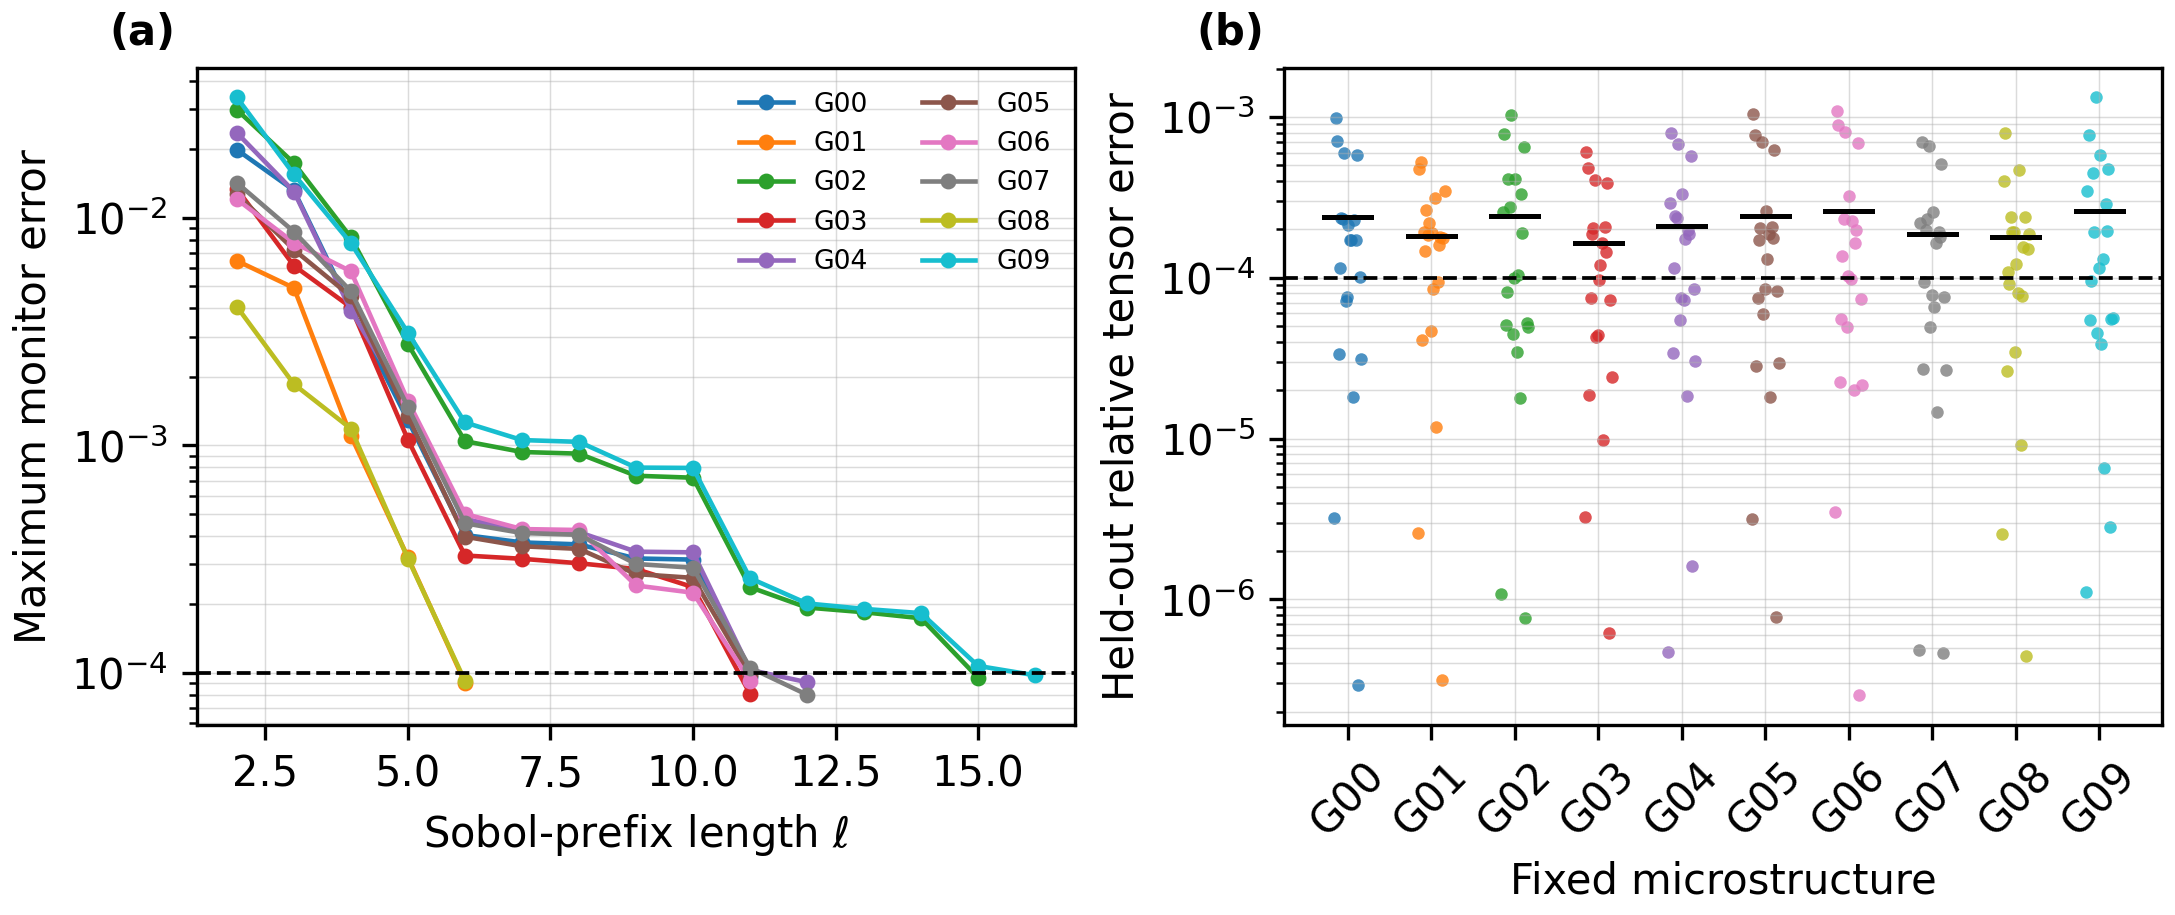
\includegraphics[width=\textwidth]{figures/numerical_adaptive_validation.png}
\captionof{figure}{Adaptive construction and independent held-out validation.
(a) Maximum monitor error during nested Sobol-prefix enrichment, with each
trajectory terminating at the first crossing of the \(0.01\%\) target.
(b) Relative errors over the 20 held-out materials for each microstructure;
horizontal segments denote microstructure-wise means. The reference level
emphasizes the distinction between the adaptive stopping tolerance and
independent held-out accuracy}
\label{fig:adaptive_validation}
\end{minipage}
\end{center}

\subsection{Controlled comparison with POD and reduced-basis models}
\label{subsec:computational_performance}
\label{subsec:pod_comparison}

A separate campaign compares G08, G00, and G09 using two independent
compilation runs per geometry, with reversed execution order in the second
repetition. The complete snapshot model is denoted full-span RB. Energy POD
and \(L^2\) POD use the same snapshot materials and all six load cases.
Their retained ranks are selected using only the same five monitor materials,
with the same \(10^{-4}\) stopping target. Snapshots and volumetric
contractions use float32; reduced algebra and the direct \(L^2\) Gram use
float64. Validation tensors are excluded from all construction decisions
and are first computed after the initial model has been frozen. Twenty common fresh material vectors give
60 material--geometry pairs; the two timing repetitions do not create
additional independent validation data.

The factorized path builds the full-span model and supplies the operators
for energy POD. POD is charged the complete construction cost plus its
selection and export stage, not merely the cost of a small eigendecomposition.
The conventional path uses incremental spatial contractions and a direct
\(L^2\) Gram product; it shares the optimized full-order solver and overlaps
Gram work with independent compilation work. A full-span control using this
second path isolates compilation from truncation. Fixed phase/orientation
hashes, material sequences, and full-order settings are retained with the
results. All device work is serialized between models; the two repetitions
are insufficient for a broad hardware performance claim.

\begin{table}[t]
\centering
\caption{Controlled construction and POD comparison. Construction times are
means of two complete measured intervals; CPU query times are means of the
two per-run medians. Maximum validation errors are reported in percent}
\label{tab:computational_performance}
\small
\setlength{\tabcolsep}{4pt}
\begin{tabular}{@{}llrrrr@{}}
\toprule
Cell & Model / compilation & Rank & Offline [s] & CPU [\si{\micro\second}] & Max. error [\%] \\
\midrule
G08 & Full-span RB / factorized & 36 & 2.255 & 21.18 & 0.09396 \\
    & Energy POD / factorized & 32 & 2.260 & 19.83 & 0.09502 \\
    & \(L^2\) POD / conventional & 31 & 2.201 & 19.83 & 0.09613 \\
G00 & Full-span RB / factorized & 66 & 30.659 & 31.51 & 0.14656 \\
    & Energy POD / factorized & 60 & 30.669 & 29.63 & 0.14875 \\
    & \(L^2\) POD / conventional & 59 & 38.891 & 29.49 & 0.15445 \\
G09 & Full-span RB / factorized & 96 & 159.413 & 47.83 & 0.14112 \\
    & Energy POD / factorized & 92 & 159.445 & 46.38 & 0.14671 \\
    & \(L^2\) POD / conventional & 94 & 232.379 & 47.62 & 0.14222 \\
\bottomrule
\end{tabular}
\end{table}

The complete construction interval starts at runtime preparation and ends at
operator export. It includes geometry preparation, training solves, five
monitor solves, contractions, normalization, and selection where applicable;
it excludes Python import/startup and held-out validation. The full-span
factorized intervals range from 2.089 to 2.420 s for G08, 29.991 to
31.326 s for G00, and 157.814 to 161.012 s for G09. Relative to the tested
conventional \(L^2\) POD path, mean construction is reduced by 21.2\% for
G00 and 31.4\% for G09, while it is 2.5\% slower for G08. This is an
implementation comparison: energy POD uses the same factorized compiler and
has nearly the same construction time with a smaller rank.

The conventional full-span controls require 2.195, 38.880, and 232.353 s
for G08, G00, and G09, respectively. Their similarity to the corresponding
\(L^2\) POD construction costs confirms that operator assembly, rather than
POD selection, dominates this difference. Re-expressing the same raw blocks
in untruncated POD coordinates preserves their output to about
\(4.3\times10^{-14}\) relative error. Independently compiled float32 blocks,
however, differ by up to \(2.76\times10^{-4}\) in relative effective-tensor
norm in these runs, explaining why nominally equivalent full-span models
need not have identical finite-precision validation errors. The G09 full-span, energy POD, and
conventional \(L^2\) POD models meet the \(10^{-4}\) Frobenius threshold
on 11, 10, and 11 of the 20 held-out materials, respectively. Small negative
Schur-gap eigenvalues also occur in this campaign (down to approximately
\(-2.0\times10^{-5}~\si{\giga\pascal}\)); positive predicted stiffness
and finite-precision upper-bound ordering remain separate checks.

\paragraph{Where the G09 construction time is spent.}
Table~\ref{tab:g09_budget} separates the measured stages. Gram work that
overlaps other work is not added a second time. Once contraction is reduced,
snapshot and monitoring solves account for about 75\% of the factorized
construction interval. Further reductions therefore require either fewer
necessary full-order materials or cheaper full-order solves, in addition to
operator-level optimizations.

\begin{table}[t]
\centering
\caption{G09 construction budget, means of two repetitions in seconds. Rounded entries may not sum exactly}
\label{tab:g09_budget}
\begin{tabular}{@{}lrr@{}}
\toprule
Stage & Full-span / factorized & \(L^2\) POD / conventional \\
\midrule
Training FOM solves & 95.052 & 94.799 \\
Monitor FOM solves & 24.901 & 24.077 \\
Affine assembly & 30.714 & 104.919 \\
Remaining non-overlapping time & 8.747 & 8.584 \\
\midrule
Complete interval & 159.413 & 232.379 \\
\bottomrule
\end{tabular}
\end{table}

\paragraph{Latency, throughput, and memory.}
The GPU construction uses an NVIDIA GeForce RTX 5070 Ti with CuPy 13.6.0 and
CUDA runtime 13.0. Isolated CPU queries include material-to-coefficient
conversion, reduced assembly, a Cholesky solve with six right-hand sides,
and tensor output, with one BLAS thread and 200 samples per model per run.
The full-span times in Table~\ref{tab:computational_performance} are therefore
latencies, not per-item GPU batch averages. For G09, synchronized batches of
1024 coefficient queries take 3.932 ms for the full-span model, 3.785 ms for
energy POD, and 3.859 ms for conventional \(L^2\) POD. These measurements
exclude one-time operator upload and are not isolated GPU query latencies.

Peak host resident memory for G09 is 36.93 GiB for factorized full-span
construction and 36.89 GiB for conventional \(L^2\) POD; sampled additional
device memory is 9.57 and 6.66 GiB, respectively. The factorized path does not
show a peak-memory reduction in this comparison. Exported G09 operators
occupy 537.5 KiB for full-span RB and 495.0 KiB for energy POD. The compact
online artifact should therefore be distinguished from the much larger
offline snapshot workspace.

For an intended query workload, amortization must use a common timing
boundary: \(N_{\mathrm{BE}}=\lceil T_{\mathrm{offline}}/
(t_{\mathrm{FOM}}-t_{\mathrm{ROM}})\rceil\), provided the denominator is
positive. Stage sums from older runs and per-item batch throughput are not
interchanged with complete construction time and isolated latency. No
universal break-even count is inferred from those mixed measurements.

\subsection{Comparison with data-only surrogates}
\label{subsec:surrogate_comparison}

Sobol--Ritz is compared with RBF interpolation and Kriging regression under
the same training and validation conditions. For each microstructure, the
three approaches are trained using exactly the same Sobol material samples and
evaluated on the same 20 held-out materials. RBF and Kriging use the 21
independent components of the effective stiffness tensor as training outputs,
whereas Sobol--Ritz uses the six corresponding microscopic response fields to
construct the transfer space. RBF and Kriging hyperparameters are selected
using training data only, as detailed in
Appendix~\ref{app:surrogate_hyperparameters}.

\begin{table}[t]
\caption{Same-prefix held-out comparison with data-only surrogates.
Relative Frobenius errors are reported in percent.}
\label{tab:surrogate_baselines}
\setlength{\tabcolsep}{4pt}
\renewcommand{\arraystretch}{1.05}
\begin{tabular}{@{}lcrrr@{\hspace{8pt}}rrr@{}}
\toprule
& &
\multicolumn{3}{c}{Mean error [\%]} &
\multicolumn{3}{c}{Maximum error [\%]} \\
\cmidrule(lr){3-5}
\cmidrule(lr){6-8}
Microstructure &
\(N_s\) &
\shortstack{Sobol--\\Ritz} &
RBF &
Kriging &
\shortstack{Sobol--\\Ritz} &
RBF &
Kriging \\
\midrule
G00 & 11 & 0.0237 & 4.15  & 5.65  & 0.0987 & 14.38 & 17.37 \\
G01 &  6 & 0.0183 & 14.22 & 12.05 & 0.0525 & 55.81 & 44.42 \\
G02 & 15 & 0.0244 & 5.09  & 3.48  & 0.103  & 18.17 & 8.35  \\
G03 & 11 & 0.0165 & 2.40  & 10.13 & 0.0605 & 6.12  & 33.54 \\
G04 & 12 & 0.0209 & 4.70  & 5.12  & 0.0793 & 17.90 & 12.30 \\
G05 & 11 & 0.0243 & 5.63  & 7.20  & 0.105  & 20.05 & 27.70 \\
G06 & 11 & 0.0260 & 6.76  & 8.01  & 0.108  & 23.84 & 19.55 \\
G07 & 12 & 0.0187 & 5.31  & 4.41  & 0.0701 & 18.59 & 10.89 \\
G08 &  6 & 0.0179 & 10.21 & 14.46 & 0.0795 & 41.39 & 54.14 \\
G09 & 16 & 0.0261 & 4.46  & 2.48  & 0.132  & 15.55 & 5.72  \\
\midrule
Overall & -- & 0.0217 & 6.29 & 7.30 & 0.132 & 55.81 & 54.14 \\
\bottomrule
\end{tabular}
\end{table}

The results in Table~\ref{tab:surrogate_baselines} show a clear separation
between Sobol--Ritz and the data-only surrogates. The aggregate mean error of Sobol--Ritz is \(0.0217\%\), compared with \(6.29\%\) for RBF and
\(7.30\%\) for Kriging; the corresponding maximum errors are \(0.132\%\),
\(55.81\%\), and \(54.14\%\), respectively. The same material samples do not imply the same training information: RBF and
Kriging use only the homogenized stiffness tensor, whereas Sobol--Ritz retains
the six microscopic response fields to construct the transfer space. This comparison measures the benefit of retaining microscopic information
and enforcing the cell equations together; it does not isolate their
individual contributions or replace the POD comparison. Moreover, the nested Sobol--Ritz
construction preserves the variational structure of the full-order problem and
provides a monotone Loewner ordering of the effective operator under nested
enrichment, a property not enforced by the data-only surrogates.

Figure~\ref{fig:surrogate_sample_efficiency} illustrates how this difference
evolves as the common training prefix increases for G03 and G09. Sobol--Ritz
maintains substantially lower held-out errors over the sampled prefixes,
showing that its advantage is already evident with small training sets.

\begin{center}
\begin{minipage}{\textwidth}
\captionsetup{hypcap=false}
\centering
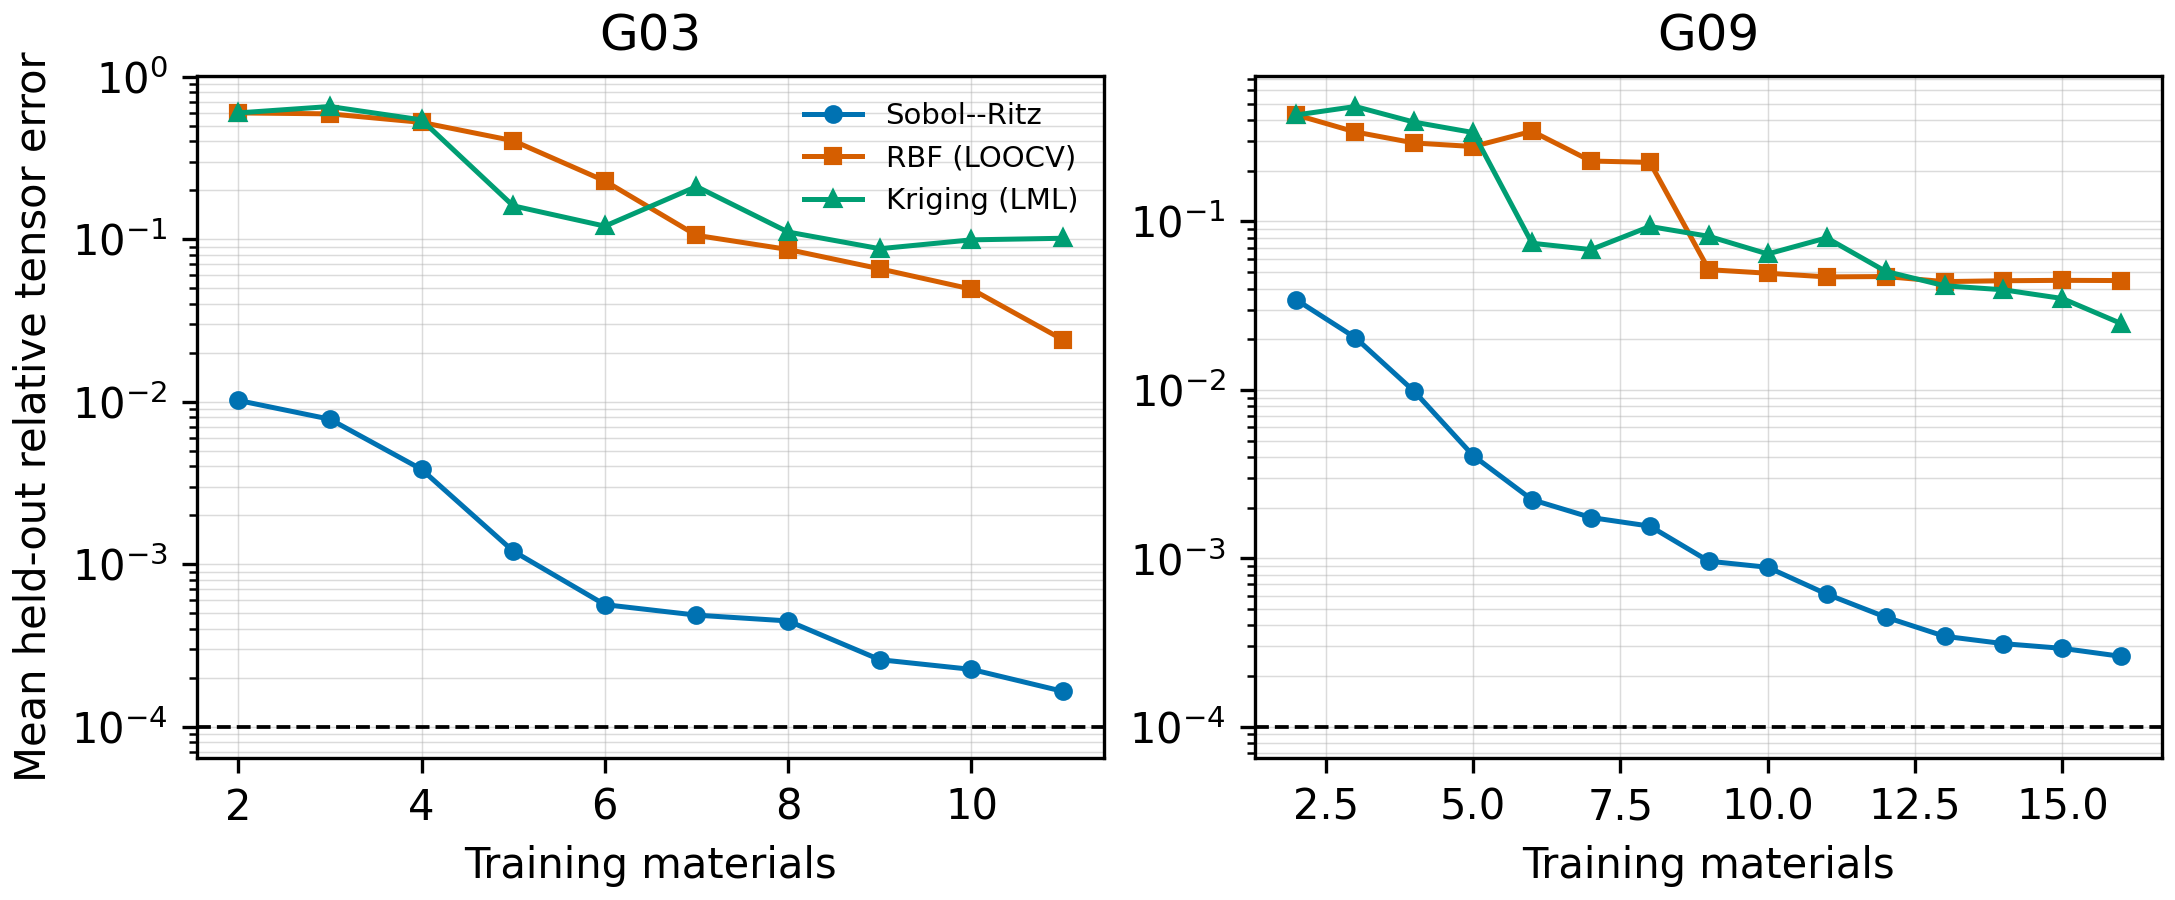
\includegraphics[width=\textwidth]{figures/numerical_surrogate_sample_efficiency.png}
\captionof{figure}{Same-prefix sample efficiency for G03 and G09.
Mean held-out relative error as the common training prefix increases.
RBF and Kriging are retuned using only the training data available at each
prefix}
\label{fig:surrogate_sample_efficiency}
\end{minipage}
\end{center}

\section{Conclusions}
\label{sec:conclusions}

This work develops and assesses an affine operator compiler for reduced-order
homogenization of voxelized linear elastic composites. Phase-supported
constitutive factors, incremental contractions, and reuse of projected
metrics reduce the spatial work required to construct the reduced operators.
The resulting Schur map is shared by full-span reduced-basis and POD models;
its established variational identities provide discrete energy diagnostics
for the implemented Galerkin models.

On ten short-fiber geometries, 6--16 snapshot materials plus five monitor
materials produce ranks of 36--96 and a mean held-out stiffness error of
0.0217\%, with maximum 0.1322\%. The maximum energy error over macroscopic
strain directions is 0.2783\% on those evaluated materials. Only 88 of the
200 material--geometry pairs meet the 0.01\% monitor tolerance. The independent
validation errors therefore characterize predictive accuracy separately from
the training stopping criterion. Voxel-resolution error remains a separate
source of uncertainty.

The controlled three-geometry comparison attributes the main measured saving
to operator compilation: complete construction is reduced by 21.2\% for G00
and 31.4\% for G09 relative to the tested conventional path, with no saving
for G08. Energy POD uses the same compiler at almost identical offline cost
and smaller rank. Isolated CPU queries require
21.18--47.83 microseconds for the full-span models. Peak offline memory
remains substantial, and no advantage over all possible POD implementations
is established.

Further development should connect these tensor-level results to a demanding
mechanical workload, extend independent spatial verification, and control
mixed-precision errors in nearly dependent contractions. Additional
controlled ablations should separate the effects of constitutive
factorization, incremental assembly, and metric reuse, using matched
precision and full-order settings. These steps would strengthen the
assessment of the compiler's practical value for repeated elastic
homogenization.

\appendix

\section{Derivation of the microscopic variational functional}
\label{app:microscopic_functional_derivation}

Consider a symmetric linear constitutive law in which the local response
associated with a field \(\boldsymbol z\) is
\[
\boldsymbol y
=
\mathbb A(\boldsymbol x;\boldsymbol\xi,\G)\boldsymbol z,
\]
where \(\boldsymbol y\) denotes the constitutively conjugate response. In
linear elasticity, for example,
\(\boldsymbol z=\boldsymbol\varepsilon\),
\(\boldsymbol y=\boldsymbol\sigma\), and
\(\mathbb A=\mathbb C\).

Because the constitutive relation is linear, the quadratic potential
associated with increasing the local field from zero to
\(\boldsymbol z\) is obtained by integrating the constitutive response along
this loading path, giving
\[
\psi(\boldsymbol z)
=
\int_{0}^{1}
\boldsymbol z^T
\mathbb A
(t\boldsymbol z)
\,\mathrm{d}t
=
\frac{1}{2}
\boldsymbol z^T
\mathbb A
\boldsymbol z.
\]
The factor \(1/2\) appears because the constitutive response increases
linearly from zero to its final value. In elasticity, this expression reduces
to the familiar strain-energy density
\(\psi=\frac{1}{2}\boldsymbol\varepsilon^T
\mathbb C\boldsymbol\varepsilon\).

Using the local-field decomposition introduced in
Eq.~\eqref{eq:local_field},
\[
\boldsymbol z(\boldsymbol x;g)
=
\overline{\boldsymbol z}(g)
+
\mathcal L u(\boldsymbol x),
\]
the local quadratic potential becomes
\[
\psi(\boldsymbol x)
=
\frac{1}{2}
\left[
\overline{\boldsymbol z}(g)
+
\mathcal L u
\right]^T
\mathbb A(\boldsymbol x;\boldsymbol\xi,\G)
\left[
\overline{\boldsymbol z}(g)
+
\mathcal L u
\right].
\]
Integrating this quantity over \(\Omega\) and dividing by the cell volume
\(|\Omega|\) gives the volume-averaged microscopic functional used in
Eq.~\eqref{eq:microscopic_energy},
\[
\Pi(u;g,\boldsymbol\xi,\G)
=
\frac{1}{2|\Omega|}
\int_{\Omega}
\left[
\overline{\boldsymbol z}(g)
+
\mathcal L u
\right]^T
\mathbb A(\boldsymbol x;\boldsymbol\xi,\G)
\left[
\overline{\boldsymbol z}(g)
+
\mathcal L u
\right]
\,\mathrm{d}\boldsymbol x.
\]

\section{Derivation of the elastic weak cell problem}
\label{app:weak_form_derivation}

For linear elasticity and in the absence of body forces, local mechanical
equilibrium inside the periodic cell is expressed in strong form as
\[
\nabla\!\cdot\!\boldsymbol\sigma=0
\qquad
\text{in }\Omega.
\]
To obtain the corresponding weak form, let
\(v\in\mathcal V_{\mathrm{per}}\) be an arbitrary admissible displacement
test function. Multiplying the equilibrium equation by \(v\), integrating
over the cell, and applying integration by parts gives
\[
-\int_{\Omega}
\boldsymbol\varepsilon(v)^T
\boldsymbol\sigma
\,\mathrm{d}\boldsymbol x
+
\int_{\partial\Omega}
v^T
\boldsymbol\sigma\boldsymbol n
\,\mathrm{d}S
=
0,
\]
where \(\boldsymbol n\) is the outward unit normal on
\(\partial\Omega\). For periodic fluctuations, the test function takes equal
values on opposite faces while the associated tractions are anti-periodic, so
the boundary contributions cancel pairwise and the remaining equilibrium
condition is
\[
\int_{\Omega}
\boldsymbol\varepsilon(v)^T
\boldsymbol\sigma
\,\mathrm{d}\boldsymbol x
=
0
\qquad
\forall v\in\mathcal V_{\mathrm{per}}.
\]

The local strain and constitutive law are
\[
\boldsymbol\varepsilon(\boldsymbol x)
=
\overline{\boldsymbol\varepsilon}
+
\boldsymbol\varepsilon(u_g),
\qquad
\boldsymbol\sigma(\boldsymbol x)
=
\mathbb C(\boldsymbol x;\boldsymbol\xi,\G)
\left[
\overline{\boldsymbol\varepsilon}
+
\boldsymbol\varepsilon(u_g)
\right],
\]
so substitution into the preceding relation yields
\[
\int_{\Omega}
\boldsymbol\varepsilon(v)^T
\mathbb C(\boldsymbol x;\boldsymbol\xi,\G)
\left[
\overline{\boldsymbol\varepsilon}
+
\boldsymbol\varepsilon(u_g)
\right]
\,\mathrm{d}\boldsymbol x
=
0
\qquad
\forall v\in\mathcal V_{\mathrm{per}}.
\]
This is the linear-elastic specialization of
Eq.~\eqref{eq:general_cell_problem}, obtained by setting
\(\mathcal L=\boldsymbol\varepsilon(\cdot)\) and
\(\mathbb A=\mathbb C\).

\section{Derivation of the discrete Schur representation}
\label{app:schur_derivation}

Starting from the microscopic functional in
Eq.~\eqref{eq:microscopic_energy}, expansion of the quadratic integrand
separates the microscopic, coupling, and macroscopic contributions as
\[
\mathcal E
=
\frac{1}{2|\Omega|}
\int_{\Omega}
(\mathcal L u)^T\mathbb A(\mathcal L u)
\,\mathrm d\boldsymbol x
+
\frac{1}{|\Omega|}
\int_{\Omega}
(\mathcal L u)^T\mathbb A\overline{\boldsymbol z}(g)
\,\mathrm d\boldsymbol x
+
\frac{1}{2|\Omega|}
\int_{\Omega}
\overline{\boldsymbol z}(g)^T
\mathbb A
\overline{\boldsymbol z}(g)
\,\mathrm d\boldsymbol x.
\]

Let \(\{\phi_a\}_{a=1}^{n}\) be a basis of the constrained discrete space
\(\mathcal V_{\mathrm{per}}^h\), so an admissible discrete fluctuation is
written as
\[
u^h(\boldsymbol x)
=
\sum_{a=1}^{n}u_a\phi_a(\boldsymbol x).
\]
Using the macroscopic loading expansion in Eq.~\eqref{eq:macro_field}, the
three blocks entering Eq.~\eqref{eq:discrete_energy} are
\begin{align*}
K_{ab}(\boldsymbol\xi;\G)
&=
\frac{1}{|\Omega|}
\int_{\Omega}
(\mathcal L\phi_a)^T
\mathbb A(\boldsymbol x;\boldsymbol\xi,\G)
(\mathcal L\phi_b)
\,\mathrm d\boldsymbol x,
\\
B_{ai}(\boldsymbol\xi;\G)
&=
-
\frac{1}{|\Omega|}
\int_{\Omega}
(\mathcal L\phi_a)^T
\mathbb A(\boldsymbol x;\boldsymbol\xi,\G)
\overline{\boldsymbol z}_i
\,\mathrm d\boldsymbol x,
\\
D_{ij}(\boldsymbol\xi;\G)
&=
\frac{1}{|\Omega|}
\int_{\Omega}
\overline{\boldsymbol z}_i^T
\mathbb A(\boldsymbol x;\boldsymbol\xi,\G)
\overline{\boldsymbol z}_j
\,\mathrm d\boldsymbol x,
\end{align*}
with \(a,b=1,\ldots,n\) and \(i,j=1,\ldots,m\). The minus sign in the
definition of \(B\) accounts for the cross-energy convention used in
Eq.~\eqref{eq:discrete_energy}.

Stationarity of Eq.~\eqref{eq:discrete_energy} with respect to \(u\) gives
\(K(\boldsymbol\xi;\G)u=B(\boldsymbol\xi;\G)g\). Collecting the \(m\)
unit-loading responses gives Eq.~\eqref{eq:fom_response}, so
\(X=K^{-1}B\) and \(u=Xg\), with the dependence on
\((\boldsymbol\xi,\G)\) understood. Substitution into the discrete energy
then gives
\[
\mathcal E(Xg,g)
=
\frac{1}{2}g^TX^TKXg
-
g^TX^TBg
+
\frac{1}{2}g^TDg.
\]
Using \(KX=B\) and \(K=K^T\) gives
\(X^TKX=X^TB=B^TX\), and therefore
\[
\mathcal E(Xg,g)
=
\frac{1}{2}
g^T
\left[
D-B^TX
\right]
g.
\]
Comparison with Eq.~\eqref{eq:effective_energy_definition} proves the Schur
representation in Eq.~\eqref{eq:schur_transfer}.

\section{Derivation of the affine discrete operators}
\label{app:affine_discrete_derivation}

The discrete affine operators in Eq.~\eqref{eq:affine_operators} follow from
the local separation in Eq.~\eqref{eq:local_affine} and the block definitions
in Appendix~\ref{app:schur_derivation}. Substituting
Eq.~\eqref{eq:local_affine} into the definition of
\(K_{ab}(\boldsymbol\xi;\G)\) gives
\[
K_{ab}(\boldsymbol\xi;\G)
=
\sum_{q=1}^{Q}
\gamma_q(\boldsymbol\xi)
\frac{1}{|\Omega|}
\int_{\Omega}
(\mathcal L\phi_a)^T
\mathbb A_q(\boldsymbol x;\G)
(\mathcal L\phi_b)
\,\mathrm d\boldsymbol x.
\]
Because \(\gamma_q(\boldsymbol\xi)\) is independent of
\(\boldsymbol x\), the remaining integral defines the fixed
microstructure-dependent block
\[
(K_q(\G))_{ab}
=
\frac{1}{|\Omega|}
\int_{\Omega}
(\mathcal L\phi_a)^T
\mathbb A_q(\boldsymbol x;\G)
(\mathcal L\phi_b)
\,\mathrm d\boldsymbol x,
\]
and therefore
\(K(\boldsymbol\xi;\G)
=\sum_q\gamma_q(\boldsymbol\xi)K_q(\G)\).
Applying the same substitution to the \(B\) and \(D\) definitions gives
\[
B(\boldsymbol\xi;\G)
=
\sum_{q=1}^{Q}
\gamma_q(\boldsymbol\xi)B_q(\G),
\qquad
D(\boldsymbol\xi;\G)
=
\sum_{q=1}^{Q}
\gamma_q(\boldsymbol\xi)D_q(\G),
\]
which completes the derivation of Eq.~\eqref{eq:affine_operators}.

\section{Nested Ritz-space ordering and monitor monotonicity}
\label{app:ritz_ordering}

This appendix proves the variational ordering stated in
Eq.~\eqref{eq:fullrank_monotone_schur} and its consequence for the monitor
error. For a fixed material--microstructure pair
\((\boldsymbol\xi,\G)\) and macroscopic loading \(g\), the FOM minimizes the
discrete energy over the complete coordinate space \(\R^n\), whereas the Ritz
approximation at enrichment step \(\ell\) minimizes the same energy over
\(\operatorname{range}(S_\ell)\). Hence,
\[
\frac{1}{2}g^T\Hfom g
=
\min_{u\in\R^n}\mathcal E(u,g),
\qquad
\frac{1}{2}g^TH_\ell^{\mathrm{eff}}g
=
\min_{u\in\operatorname{range}(S_\ell)}\mathcal E(u,g),
\]
where the dependence on \((\boldsymbol\xi,\G)\) is suppressed for
readability.

Appending a new Sobol response block preserves every previously retained
direction, so Eq.~\eqref{eq:fullrank_nested_spaces} gives
\(\operatorname{range}(S_\ell)\subseteq
\operatorname{range}(S_{\ell+1})\). Minimization over these nested spaces
therefore yields, for every \(g\in\R^m\),
\[
\frac{1}{2}g^T\Hfom g
\leq
\frac{1}{2}g^TH_{\ell+1}^{\mathrm{eff}}g
\leq
\frac{1}{2}g^TH_\ell^{\mathrm{eff}}g,
\]
which is equivalent to the Loewner ordering
\[
\Hfom
\preceq
H_{\ell+1}^{\mathrm{eff}}
\preceq
H_\ell^{\mathrm{eff}}.
\]
This proves Eq.~\eqref{eq:fullrank_monotone_schur}.

To connect this matrix ordering with the scalar monitor error, define
\(\Delta_\ell=H_\ell^{\mathrm{eff}}-\Hfom\) and
\(\Delta_{\ell+1}=H_{\ell+1}^{\mathrm{eff}}-\Hfom\). The preceding result
gives
\(0\preceq\Delta_{\ell+1}\preceq\Delta_\ell\), so
\(E=\Delta_\ell-\Delta_{\ell+1}\succeq0\). The difference between the
squared Frobenius norms is then
\[
\|\Delta_\ell\|_F^2-
\|\Delta_{\ell+1}\|_F^2
=
2\operatorname{tr}(\Delta_{\ell+1}E)
+
\operatorname{tr}(E^2)
\geq0,
\]
because the trace of the product of two positive-semidefinite matrices is
nonnegative. Thus,
\(\|\Delta_{\ell+1}\|_F\leq\|\Delta_\ell\|_F\). Since the FOM denominator
in Eq.~\eqref{eq:monitor_stopping} is fixed for each monitor material, its
relative error is non-increasing under nested enrichment, and taking the
maximum over the fixed set \(\Xi_M\) gives
\(e_M^{(\ell+1)}\leq e_M^{(\ell)}\) in exact arithmetic.

\section{Derivation of the Ritz--Schur error identity}
\label{app:ritz_schur_identity_derivation}

Consider a fixed material--microstructure pair \((\boldsymbol\xi,\G)\) and
suppress this dependence for readability. Let
\[
\Delta X=X-X_r\in\R^{n\times m},
\qquad
R=B-KX_r\in\R^{n\times m}.
\]
Using the full-order equation \(KX=B\) gives
\[
R
=
KX-KX_r
=
K\Delta X,
\]
and, because \(K\) is symmetric positive definite and therefore invertible,
\(\Delta X=K^{-1}R\).

From the full-order and reduced Schur maps in
Eqs.~\eqref{eq:schur_transfer} and \eqref{eq:reduced_transfer},
\[
\Hr-\Hfom
=
\left(D-B^TX_r\right)-\left(D-B^TX\right)
=
B^T\Delta X.
\]
Using \(B=KX=K(X_r+\Delta X)\) and \(K=K^T\) gives
\[
B^T\Delta X
=
X_r^TK\Delta X
+
(\Delta X)^TK(\Delta X).
\]
The Galerkin condition associated with Eq.~\eqref{eq:reduced_response} is
\(V_r^T(KX_r-B)=0\), or equivalently \(V_r^TR=0\). Since
\(X_r=V_r\widehat X_r\) and \(K\Delta X=R\), the cross term vanishes,
\[
X_r^TK\Delta X
=
\widehat X_r^TV_r^TR
=
0,
\]
so
\[
\Hr-\Hfom
=
(\Delta X)^TK(\Delta X).
\]
Substituting \(\Delta X=K^{-1}R\) and using the symmetry of \(K\) gives
\[
(\Delta X)^TK(\Delta X)
=
R^TK^{-1}R.
\]
Finally, for every \(g\in\R^m\),
\[
g^T(\Hr-\Hfom)g
=
(\Delta Xg)^TK(\Delta Xg)
\geq0,
\]
which proves the exact identity and positive-semidefinite ordering in
Eq.~\eqref{eq:ritz_schur_identity}.

\section{Elasticity-specific affine constitutive representation}
\label{app:affine}

This appendix specializes the general affine separation of
Eq.~\eqref{eq:local_affine} to the elastic material family defined in
Eq.~\eqref{eq:elastic_material_vector}. Let
\(\chi_m(\boldsymbol x)\) and \(\chi_f(\boldsymbol x)\) denote the matrix and
fiber indicator functions, with \(\chi_m+\chi_f=1\).

For the isotropic matrix, the Lam\'e parameters are
\[
\mu_m
=
\frac{E_m}{2(1+\nu_m)},
\qquad
\lambda_m
=
\frac{E_m\nu_m}{(1+\nu_m)(1-2\nu_m)}.
\]
The corresponding Mandel stiffness is represented by the two fixed basis
matrices in Eq.~\eqref{eq:matrix_affine_basis}:
\begin{equation}
\label{eq:matrix_affine_basis}
\begin{aligned}
C_m
&=
\lambda_m M^{(m)}_1
+
\mu_m M^{(m)}_2\\
&=
\begin{bmatrix}
\lambda_m+2\mu_m & \lambda_m & \lambda_m & 0 & 0 & 0\\
\lambda_m & \lambda_m+2\mu_m & \lambda_m & 0 & 0 & 0\\
\lambda_m & \lambda_m & \lambda_m+2\mu_m & 0 & 0 & 0\\
0&0&0&2\mu_m&0&0\\
0&0&0&0&2\mu_m&0\\
0&0&0&0&0&2\mu_m
\end{bmatrix}
\in\R^{6\times6}.
\end{aligned}
\end{equation}

The fiber is transversely isotropic about its local longitudinal axis. From
the five independent engineering constants in
Eq.~\eqref{eq:elastic_material_vector},
\[
G_{TT}
=
\frac{E_T}{2(1+\nu_{TT})},
\qquad
\nu_{TL}
=
\nu_{LT}\frac{E_T}{E_L}.
\]
Using the Mandel ordering
\((11,22,33,\sqrt{2}\,23,\sqrt{2}\,13,\sqrt{2}\,12)\), the local fiber
compliance is defined in Eq.~\eqref{eq:fiber_local_compliance} as
\begin{equation}
\label{eq:fiber_local_compliance}
\mathbb S_f^{\mathrm{loc}}
=
\begin{bmatrix}
\dfrac{1}{E_L} & -\dfrac{\nu_{LT}}{E_L} & -\dfrac{\nu_{LT}}{E_L} & 0&0&0
\\[2mm]
-\dfrac{\nu_{LT}}{E_L} & \dfrac{1}{E_T} & -\dfrac{\nu_{TT}}{E_T} & 0&0&0
\\[2mm]
-\dfrac{\nu_{LT}}{E_L} & -\dfrac{\nu_{TT}}{E_T} & \dfrac{1}{E_T} & 0&0&0
\\[2mm]
0&0&0&\dfrac{1}{2G_{TT}}&0&0
\\[2mm]
0&0&0&0&\dfrac{1}{2G_{LT}}&0
\\[2mm]
0&0&0&0&0&\dfrac{1}{2G_{LT}}
\end{bmatrix}
\in\R^{6\times6}.
\end{equation}

The local stiffness is
\(C_f^{\mathrm{loc}}=(\mathbb S_f^{\mathrm{loc}})^{-1}\). Transverse isotropy
gives the five-coefficient representation in
Eq.~\eqref{eq:fiber_local_stiffness}:
\begin{equation}
\label{eq:fiber_local_stiffness}
C_f^{\mathrm{loc}}
=
\begin{bmatrix}
c_1 & c_2 & c_2 & 0 & 0 & 0\\
c_2 & c_3 & c_4 & 0 & 0 & 0\\
c_2 & c_4 & c_3 & 0 & 0 & 0\\
0 & 0 & 0 & c_3-c_4 & 0 & 0\\
0 & 0 & 0 & 0 & c_5 & 0\\
0 & 0 & 0 & 0 & 0 & c_5
\end{bmatrix}
=
\sum_{j=1}^{5}
c_j(\boldsymbol\xi)M^{(f)}_j
\in\R^{6\times6}.
\end{equation}
The coefficients \(c_j(\boldsymbol\xi)\) follow directly from the inverse of
Eq.~\eqref{eq:fiber_local_compliance}, while the matrices \(M_j^{(f)}\) are
fixed.

Let \(\mathcal T(\boldsymbol x;\G)\in\R^{6\times6}\) denote the
energy-preserving Mandel rotation associated with the local fiber direction.
Combining the matrix and fiber phases gives the local stiffness field defined
in Eq.~\eqref{eq:elastic_local_field}:
\begin{equation}
\label{eq:elastic_local_field}
\mathbb C(\boldsymbol x;\boldsymbol\xi,\G)
=
\chi_m(\boldsymbol x)C_m
+
\chi_f(\boldsymbol x)
\mathcal T(\boldsymbol x;\G)
C_f^{\mathrm{loc}}
\mathcal T(\boldsymbol x;\G)^T
\in\R^{6\times6}.
\end{equation}

Substituting Eqs.~\eqref{eq:matrix_affine_basis} and
\eqref{eq:fiber_local_stiffness} into
Eq.~\eqref{eq:elastic_local_field} gives the exact elasticity-specific
separation defined in Eq.~\eqref{eq:elastic_affine_expansion}:
\begin{equation}
\label{eq:elastic_affine_expansion}
\mathbb C(\boldsymbol x;\boldsymbol\xi,\G)
=
\sum_{q=1}^{7}
\gamma_q(\boldsymbol\xi)
\mathbb A_q(\boldsymbol x;\G).
\end{equation}
The corresponding coefficient vector is defined in
Eq.~\eqref{eq:elastic_gamma} as
\begin{equation}
\label{eq:elastic_gamma}
\boldsymbol\gamma(\boldsymbol\xi)
=
\left[
\lambda_m,\,
\mu_m,\,
c_1,\,
c_2,\,
c_3,\,
c_4,\,
c_5
\right]^T
\in\R^7,
\qquad
Q=7.
\end{equation}
The associated fixed spatial fields are
\[
\mathbb A_1
=
\chi_m M^{(m)}_1,
\qquad
\mathbb A_2
=
\chi_m M^{(m)}_2,
\]
and, for \(j=1,\ldots,5\),
\[
\mathbb A_{2+j}(\boldsymbol x;\G)
=
\chi_f(\boldsymbol x)
\mathcal T(\boldsymbol x;\G)
M^{(f)}_j
\mathcal T(\boldsymbol x;\G)^T.
\]
Thus, the queried material changes only the seven coefficients in
Eq.~\eqref{eq:elastic_gamma}, while the phase distribution and local
orientations remain fixed in \(\mathbb A_q(\boldsymbol x;\G)\). These fields
generate the reusable discrete blocks in Eq.~\eqref{eq:affine_operators}.

\section{Voxel-resolution convergence}
\label{app:voxel_resolution}

The adopted voxel resolution is assessed using three representative
microstructures spanning the considered ranges of fiber volume fraction and
aspect ratio: G08, G00, and G09. For each microstructure, the same continuous
fiber realization is rasterized at 3, 4, 5, and 6 voxels per fiber diameter,
thereby isolating the effect of spatial discretization.

The constituent properties used for this resolution study correspond to the
Carbon Fiber (290 GPa)/Resin Epoxy system from the ANSYS Composite Materials
Sample Library \cite{AnsysCompositeMaterials}: \(E_m=3.78~\si{\giga\pascal}\),
\(\nu_m=0.35\), \(E_L=290~\si{\giga\pascal}\),
\(E_T=23~\si{\giga\pascal}\), \(G_{LT}=9~\si{\giga\pascal}\),
\(\nu_{LT}=0.20\), and \(\nu_{TT}=0.40\). These values lie within the
constitutive domain defined in Table~\ref{tab:material_domain}. The library
provides constituent data; the cell calculations use the FFT solver described
in this work.

Taking the result at 6 voxels per fiber diameter as reference, the resulting
relative effective-stiffness differences are summarized in
Table~\ref{tab:voxel_resolution_details}.

\begin{table}[htbp]
\caption{Relative effective-stiffness difference
\(100e_\rho\) (\%) with respect to 6 voxels per fiber diameter.}
\label{tab:voxel_resolution_details}
\begin{tabular}{@{}lrrrr@{}}
\toprule
& \multicolumn{4}{c}{Resolution [voxels/diameter]} \\
\cmidrule(lr){2-5}
Microstructure & 3 & 4 & 5 & 6 \\
\midrule
G08 & 0.140 & 0.0935 & 0.0993 & 0 \\
G00 & 2.494 & 1.160  & 0.384  & 0 \\
G09 & 5.383 & 2.998  & 0.910  & 0 \\
\bottomrule
\end{tabular}
\par\smallskip
\footnotesize\textit{Note:} \(\rho\in\{3,4,5,6\}\) denotes the resolution in
voxels per fiber diameter, and
\(e_\rho=\|C_\rho^{\mathrm{eff}}-C_6^{\mathrm{eff}}\|_F/
\|C_6^{\mathrm{eff}}\|_F\).
\end{table}

At 5 voxels per fiber diameter, the differences relative to the
6-voxel reference are \(0.0993\%\), \(0.384\%\), and \(0.910\%\) for
G08, G00, and G09, respectively. The numerical campaign therefore adopts
6 voxels per fiber diameter as a common discretization level.

\section{Training-only surrogate hyperparameter selection}
\label{app:surrogate_hyperparameters}

The RBF and Kriging comparisons use the same Sobol prefix available to the
transfer model at each training size. Inputs are the seven affine
constitutive coefficients, normalized coordinatewise using ranges computed
from the fixed 1024-point candidate sequence. Outputs are the 21 independent
upper-triangular entries of the symmetric Mandel stiffness tensor and are
standardized using only the current training prefix.

For RBF, deterministic leave-one-out cross-validation minimizes the mean
relative Frobenius tensor error over eight kernel families: linear,
thin-plate, cubic, quintic, multiquadric, inverse-multiquadric,
inverse-quadratic, and Gaussian. The shape parameter spans 16 logarithmically
spaced multiples from \(2^{-12}\) to \(2^3\) of the inverse median pair
distance. Five smoothing levels from zero to \(10^{-1}\) and every polynomial
degree admissible at the current fold size are also considered.

For Kriging, the covariance family is selected by maximum optimized training
log marginal likelihood among ten isotropic and
automatic-relevance-determination variants of Mat\'ern,
squared-exponential, rational-quadratic, and Mat\'ern-plus-linear kernels.
Covariance amplitude, length scales, nugget, and the rational-quadratic shape
parameter when applicable are optimized continuously. Every candidate uses
two deterministic optimizer restarts during family selection; the winning
family is then refitted with ten deterministic restarts. This complete search
is repeated for every microstructure and prefix. Monitor and held-out responses
are excluded from all hyperparameter decisions.

\section*{Statements and Declarations}

\subsection*{Funding}
This work was supported by Escuela Polit\'ecnica Nacional [grant number
PIGR-2401] and the VLIR-UOS organization [grant number
PIEX-DIM-VLIR-25 (EC2024TEA547A101)].

\subsection*{Competing interests}
The authors declare that they have no known competing financial interests or
personal relationships that could have appeared to influence the work
reported in this paper.

\subsection*{Author contributions}
Kevin Vidal: conceptualization, methodology, software, formal analysis,
investigation, data curation, visualization, and writing the original draft.
Victor Alulema: conceptualization, methodology, validation, formal analysis,
investigation, and review and editing. Victor Berrazueta: validation,
resources, and review and editing. Esteban Valencia: supervision, project
administration, resources, and review and editing.

\subsection*{Data and code availability}
The numerical data were generated computationally. The working project
contains the geometry definitions, material sequences, full-order and reduced
solvers, frozen operator artifacts, and validation and timing records.
% AUTHOR ACTION BEFORE SUBMISSION: specify the accessible archival repository,
% release/commit, license, and any restrictions. A public release has not yet
% been established; do not replace this with an invented DOI or availability promise.
A persistent public release location is not yet specified in this draft.

\subsection*{AI-assisted work}
OpenAI Codex was used to assist with code development, numerical audit scripts,
and manuscript restructuring. This assistance does not constitute independent
scientific validation.
% AUTHOR ACTION BEFORE SUBMISSION: confirm the complete disclosure and verify
% the assisted material, results, attribution, and references. Do not claim
% coauthor verification before it has occurred.

\subsection*{Author identifiers}
Kevin Vidal: \url{https://orcid.org/0009-0006-8667-4525};
Victor Alulema: \url{https://orcid.org/0000-0001-7351-5281};
Victor Berrazueta: \url{https://orcid.org/0009-0005-8405-6208};
Esteban Valencia: \url{https://orcid.org/0000-0002-6496-9908}.

\bibliography{references_cmame}

\end{document}
